\documentclass[12pt, a4paper]{article}

\usepackage{fontspec}
\usepackage[english]{babel}
\usepackage{sectsty}
\usepackage{natbib}
\usepackage{float}
\usepackage{parskip}
\usepackage{graphicx}
\usepackage{titlesec}
\usepackage{titletoc}
\usepackage[nottoc]{tocbibind} 
\usepackage{ragged2e}
\usepackage{enumitem}
\usepackage[top=1in, bottom=1in, right=1in, left=1in]{geometry}
\usepackage{tocloft}
% un comment below make ToC entires into links
% \usepackage{hyperref}
% for line height
\usepackage{setspace}
% \usepackage{etoolbox}

%% For dummy text
\usepackage[english]{babel}
\usepackage{blindtext}

% Required for the math packages used in Section 3.2.3
\usepackage{amsmath}
\usepackage{amssymb}

\usepackage{url}

\usepackage{hyperref}
\hypersetup{
    colorlinks = true,
    linkcolor = black,
    citecolor = black,
    urlcolor = blue,
    bookmarks = true
}




\counterwithin{figure}{section}
\renewcommand\cftloftitlefont{\normalfont\ssecfnt\bfseries}
\renewcommand{\cftlottitlefont}{\normalfont\ssecfnt\bfseries}
\renewcommand{\cfttoctitlefont}{\normalfont\ssecfnt\bfseries}
% \setlength{\cftsecnumwidth}{65pt}%
% \renewcommand{\cftchappresnum}{\chaptername\hspace{5pt}}
% \renewcommand{\cftchapaftersnum}{\hspace{5pt}}

%set font of section including toc, lof, lot
\renewcommand{\cftsecfont}{\normalfont\ssecfnt}

% List of equations
\newcommand{\listequationsname}{\normalfont\ssecfnt\bfseries List of Equations}
\newlistof{myequations}{equ}{\listequationsname}
\newcommand{\myequations}[1]{%
\addcontentsline{equ}{myequations}{\protect\numberline{\theequation}#1}\par}

\newcommand{\secfnt}{\fontsize{14}{16}\selectfont}
\newcommand{\ssecfnt}{\fontsize{12}{14}\selectfont}

%%% FORMAT TITLES %%%
\titleformat{\section}
{\normalfont\secfnt\bfseries\centering}{Chapter~\thesection:}{0.5em}{}

\titleformat{\subsection}
{\normalfont\ssecfnt\bfseries}{\thesubsection}{1em}{}

\titleformat{\subsubsection}
{\normalfont\ssecfnt\bfseries}{\thesubsubsection}{1em}{}
\titleformat{\paragraph}
{\normalfont\ssecfnt\bfseries}{\theparagraph}{1em}{}
\titlespacing*{\paragraph}{0pt}{10pt}{6pt}
%%% END FORMAT TITLES %%%

%%% FORMAT TITLES IN TOC %%%
\setmonofont{Times New Roman}
\titlecontents{section}[3.5em]{\normalfont}%
{\contentslabel[Chapter \thecontentslabel:]{3em}\qquad}%numbered
{\hskip-3em}%numberless
{\titlerule*[0.75pc]{.}\contentspage}%
\renewcommand{\cftsecaftersnum}{\hspace{5pt}}
%%% END FORMAT TITLES IN TOC %%%

%%% CONTROL SPACING AFTER HEADINGS %%%
\titlespacing*{\section}{0pt}{18pt}{10pt}
\titlespacing*{\subsection}{0pt}{14pt}{8pt}
\titlespacing*{\subsubsection}{0pt}{12pt}{6pt}
%%% END CONTROL SPACING AFTER HEADINGS %%%

\graphicspath{ {./images/} }

%%% CHANGE NAME OF TOC %%%
\addto\captionsenglish{
  \renewcommand{\contentsname}{Table of Contents}
}
%%% END CHANGE NAME OF TOC %%%

%%% SET MAIN FONT FAMILY %%%
\setmainfont{Times New Roman}
%%% END SET MAIN FONT FAMILY %%%

\setstretch{1.5}

% \renewcommand{\cftsec}{}

\begin{document}
\justifying
\begin{center}
    \textbf{Smart Drainage Monitoring and Flood Prediction System for Urban Areas in Kenya (Capstone)\\
    \vspace{50pt}
    Njenga Martin Njuguna\\
    165852\\
    ICS 4D\\
    \vspace{70pt}
    Supervisor:\\
    Ouma, Kelvin\\
    \vspace{70pt}
    An Informatics and Computer Science Project Proposal Submitted to the School of Computing and Engineering Sciences in partial fulfillment of the requirements for the award of a Degree in Bachelor of Science in Informatics and Computer Science \\
    \vspace{70pt}
    School of Computing and Engineering Science\\
    Strathmore University\\
    Nairobi, Kenya\\
    \vspace{50pt}
    July 2026
     }
\end{center}

\thispagestyle{empty}
\clearpage
\pagenumbering{roman}
\section*{Declaration and Approval}
\addcontentsline{toc}{section}{Declaration and Approval}
I declare that this project proposal has not been submitted to Strathmore University or any other University for the award of a Degree in Bachelor of Science in Informatics and Computer Science or any other Degree. To the best of my knowledge and belief, the research proposal contains no material previously published or written by another person except where due reference is made in the research proposal itself.  

\vspace{2cm}

Admission Number: 165852

\vspace{1cm}

Student Signature:
\raisebox{-0.3cm}{
\includegraphics[height=1.5cm]{Images/signature.png}}
\hspace{-2.5cm}
\underline{\hspace{3.5cm}}
\hspace{1cm}
Date: \underline{\makebox[3.5cm][c]{11/06/2026}}

\vspace{2cm}

Supervisor Signature:
\underline{\hspace{3.5cm}}
\hspace{1cm}
Date: \underline{\makebox[3.5cm][c]{12/06/2026}}

\vspace{2cm}

\clearpage
\section*{Acknowledgement}
\addcontentsline{toc}{section}{Acknowledgement}
I would like to express my heartfelt gratitude to my supervisor,Mr. Ouma Kelvin, for his guidance, constructive feedback, and continued support throughout the development of this project proposal. His insights and direction have been invaluable in shaping the scope and depth of this research.
Finally, I acknowledge the contributions of the researchers and authors whose published works have informed and supported the literature review and technical design presented in this proposal.
\clearpage
\section*{Abstract}
\addcontentsline{toc}{section}{Abstract}

Urban flooding remains a critical challenge in Nairobi, Kenya, where
inadequate drainage infrastructure, reactive management practices,
and the absence of real-time monitoring systems continue to cause
loss of life and destruction of property. This study presents the
design and development of a Smart Drainage Monitoring and Flood
Prediction System implemented as a hardware-software prototype
integrating distributed IoT sensor nodes with a multi-model machine
learning pipeline and a web-based monitoring dashboard.

The system deploys ESP32 microcontrollers interfaced with ultrasonic
water level sensors, flow rate sensors, and MQ-series gas sensors
transmitting data via MQTT to a centralised platform. A three-stage
machine learning pipeline processes incoming sensor readings
sequentially. First, an Isolation Forest algorithm performs anomaly
detection by identifying significant deviations from established
baseline drainage conditions, flagging unusual water level spikes,
unexpected flow rate drops, and abnormal gas concentration readings
that may indicate developing blockages or flood risk. Second, a
Random Forest model classifies the current drainage state as Normal,
Blockage Risk, or Flood Risk. Third, an LSTM network predicts future
water levels and estimates time to critical flood thresholds based
on historical sensor trends. Blockages are identified through
sustained flow rate differentials between consecutive monitoring
nodes.

Training data for the machine learning models is sourced from the
UCI Machine Learning Repository, Kaggle, the Global Runoff Data
Centre, and Zenodo, supplemented by simulated prototype sensor
data. The study follows a mixed exploratory and experimental
research paradigm, applying the CRISP-DM methodology for the
machine learning pipeline and Agile Scrum for system development.
The system is evaluated through controlled prototype testing against
predefined metrics including classification accuracy, anomaly
detection recall, and LSTM prediction error, contributing a prototype that demonstrates technical feasibility toward proactive urban drainage management in Kenya.


\clearpage

\begin{center}
    \tableofcontents
    \clearpage
\end{center}
%
\begin{center}
    \listoffigures
    \clearpage
\end{center}
%
\begin{center}
    \listoftables
    \clearpage
\end{center}
%

\addcontentsline{toc}{section}{List of Abbreviations}
\section*{List of Abbreviations}
\begin{description}[leftmargin=3cm, style=nextline]
    \item[ESP32] Espressif Systems 32-bit: A low-cost, 
    low-power microcontroller with built-in Wi-Fi and Bluetooth 
    capabilities, used in this study as the core processing unit 
    for distributed sensor nodes within the drainage monitoring 
    system.

    \item[IoT] Internet of Things: A network of interconnected 
    physical devices embedded with sensors, software, and 
    communication capabilities that enable them to collect and 
    exchange data over the internet or local networks.

    \item[JICA] Japan International Cooperation Agency: A Japanese 
    government agency responsible for coordinating official 
    development assistance and technical cooperation projects in 
    developing countries, including urban planning initiatives 
    in Kenya.

    \item[LSTM] Long Short-Term Memory: A type of recurrent neural 
    network architecture designed to learn patterns from sequential 
    and time-series data, used in this study for predicting future 
    water levels and estimating time to critical flood thresholds 
    based on historical sensor readings.

    \item[ML] Machine Learning: A branch of artificial intelligence 
    in which computer systems are trained to learn patterns from 
    data and make decisions or predictions without being explicitly 
    programmed for each task.

    \item[MQTT] Message Queuing Telemetry Transport: A lightweight, 
    publish-subscribe network communication protocol designed for 
    constrained devices and low-bandwidth environments, used in 
    this study for real-time transmission of sensor data between 
    distributed monitoring nodes and the centralized monitoring 
    platform.

    \item[NIUPLAN] Nairobi Integrated Urban Development Master Plan: 
    A comprehensive urban development framework developed jointly 
    by the Japan International Cooperation Agency and Nairobi City 
    County to guide the long-term physical, economic, and 
    infrastructure development of Nairobi.

    \item[RF] Random Forest: A supervised machine learning algorithm 
    that constructs multiple decision trees during training and 
    combines their outputs to classify data into predefined 
    categories, used in this study to classify drainage conditions 
    as Normal, Blockage Risk, or Flood Risk.

    \item[CH$_4$]
    Methane: A flammable and potentially explosive gas that can
    accumulate within enclosed drainage channels as a byproduct of
    the decomposition of organic waste materials.

    \item[GSM]
    Global System for Mobile Communications: A standard for
    mobile communication networks used for SMS-based alert
    transmission in IoT and sensor network systems.
 
    \item[H$_2$S]
    Hydrogen Sulfide: A toxic and corrosive gas produced by the
    anaerobic decomposition of organic materials within drainage
    channels, posing significant health risks to maintenance
    personnel.

    \item[MAE]
    Mean Absolute Error: A regression evaluation metric that
    measures the average absolute difference between predicted
    and actual values, used to assess LSTM water level prediction
    performance.

    \item[MQ]
    Metal Oxide: A family of gas sensor modules commonly used in
    IoT systems for detecting the concentration of specific gases
    such as methane, hydrogen sulfide, and ammonia in the
    surrounding environment.
 
    \item[NH$_3$]
    Ammonia: A toxic gas produced by the decomposition of organic
    waste within drainage channels, monitored in this system to
    protect maintenance personnel from harmful exposure.

    \item[NRF]
    Nordic Radio Frequency: A family of low-power wireless
    communication modules used for short-range node-to-node
    data transmission in sensor network deployments.
 
    \item[ppm]
    Parts Per Million: A unit of concentration used to express
    the amount of a gas present in air, used in this study to
    report sensor readings for methane, hydrogen sulfide, and
    ammonia concentrations within drainage channels.
    

\end{description}
\clearpage
\pagenumbering{arabic}
\section{Introduction}
\subsection{Background Information}

Flooding has become one of the major environmental and infrastructural challenges affecting many urban areas across the world, especially in rapidly growing cities where drainage systems are unable to adequately support the increasing population and urban development. In Kenya, heavy rainfall seasons frequently result in severe flooding that leads to destruction of roads, disruption of transport systems, displacement of residents, environmental pollution, and loss of lives. According to \citet{avery2024}, floods experienced in Kenya between March and April 2024 caused the deaths of at least 169 people, with Nairobi being among the most affected urban areas. Although flooding is a natural occurrence, its effects have become more severe due to poor urban planning, blocked drainage systems, encroachment into riparian areas, and inadequate maintenance of stormwater infrastructure.

Rapid urbanization in Nairobi has significantly increased pressure on existing drainage systems. As urban areas expand, natural land surfaces are increasingly replaced by buildings, roads, and pavements that prevent water infiltration into the soil, resulting in increased surface runoff during rainfall. Studies on urban resilience in Nairobi established that the growth of impermeable surfaces has directly contributed to increased urban flooding and drainage overload \citep{nyamumbo2025}. Informal settlements and densely populated urban regions are particularly vulnerable because they often lack proper drainage infrastructure and waste management systems. Solid waste disposal into drainage channels further contributes to blockage of water flow, causing stormwater to overflow into roads, residential areas, and business premises.

Current drainage management approaches in many urban areas within Kenya are largely reactive rather than preventive. Maintenance activities are commonly performed after flooding has already occurred, making it difficult for authorities to effectively respond to emerging drainage issues before they escalate into disasters. The Nairobi Integrated Urban Development Master Plan (NIUPLAN) highlights that Nairobi’s drainage and sewerage systems have not kept pace with rapid urban growth and are increasingly unable to manage heavy stormwater flows effectively \citep{jica2014}.
\clearpage
\subsection{Problem Statement}

Urban flooding has become one of the most persistent and damaging challenges facing rapidly growing cities in Kenya, particularly Nairobi, where inadequate drainage infrastructure, poor waste management practices, and unplanned urban expansion continue to overwhelm existing stormwater systems. Despite the severity and frequency of flooding events in Nairobi, drainage management within the city remains largely reactive, relying on manual inspections and maintenance activities that are only carried out after flooding has already occurred. This means that county authorities and disaster management agencies are consistently unable to detect and respond to drainage problems before they escalate into full flooding disasters.

A major contributor to urban flooding in Nairobi is the blockage of drainage channels caused by the disposal of solid waste into drainage networks. As waste accumulates within drainage channels, water flow is gradually restricted, causing stormwater to overflow into roads, residential areas, and business premises during heavy rainfall. Currently, there are no automated systems in place to continuously monitor flow conditions within drainage channels and detect early signs of blockage before overflow occurs. As a result, blockages are typically only identified after they have already caused flooding, making timely intervention difficult for maintenance teams.

Beyond the challenge of physical blockages and flooding, urban drainage channels also present a serious but often overlooked environmental and public health hazard. The decomposition of organic waste materials that accumulate within drainage systems generates harmful gases including methane, hydrogen sulfide, and ammonia. These gases can accumulate within enclosed or partially enclosed drainage channels to dangerous concentrations, posing significant health risks to residents living near drainage infrastructure and to maintenance personnel working within or around drainage channels. Existing drainage systems in Kenya lack any mechanism for continuously monitoring the presence and concentration of such gases, leaving both the public and workers exposed to potential harm without warning.

Furthermore, the absence of data-driven tools for analyzing drainage conditions means that there is currently no reliable way to predict flooding events before they occur. Flood prediction requires continuous collection and analysis of data on water levels and flow rates across multiple points within a drainage network. Without such data, emergency response agencies are forced to act on flooding only after it has already caused damage, rather than being able to issue early warnings and take preventive action in advance.

Therefore, there exists a clear need for an intelligent drainage monitoring system capable of continuously collecting real-time data on water levels, water flow rates, drainage blockages, and harmful gas concentrations within urban drainage channels. Such a system should be capable of analyzing collected sensor data using machine learning techniques to detect anomalies, identify possible blockages, predict potential flooding events, and generate timely early warning alerts for county authorities and disaster management agencies in Kenya.

\subsection{General Objective}

To develop a smart drainage monitoring and flood prediction system for urban areas in Kenya.
\subsubsection{Specific Objectives}

\begin{enumerate}[label=\roman*.]

\item To investigate the challenges associated with existing
urban drainage management practices in Kenya through a review
of related literature.

\item To critically review existing technological tools and
systems developed to address urban drainage monitoring and
flood management challenges and identify their limitations.

\item To design and develop a distributed sensor-based framework
for collecting real-time data on water levels, flow rates,
drainage blockages, and harmful gas concentrations within
urban drainage channels.

\item To develop and evaluate the effectiveness of a machine
learning pipeline incorporating Isolation Forest-based
detection of anomalous sensor deviations, Random Forest
drainage state classification, and LSTM-based flood risk
prediction using sensor data from publicly available
drainage and flood datasets.

\item To evaluate the performance and reliability of the
proposed smart drainage monitoring and flood prediction
system through prototype testing against predefined
performance metrics including classification accuracy,
anomaly detection recall, and LSTM prediction error.

\end{enumerate}

\subsubsection{Research Questions}

\begin{enumerate}[label=\roman*.]

\item What are the challenges associated with existing urban
drainage management practices in Kenya?

\item What existing technological tools and systems have been
developed to address urban drainage monitoring and flood
management challenges, and what are their limitations?

\item How can a distributed sensor-based framework be designed
and developed to collect real-time data on water levels,
flow rates, drainage blockages, and harmful gas
concentrations within urban drainage channels?

\item How can a machine learning pipeline incorporating
Isolation Forest-based detection of anomalous sensor
deviations, Random Forest drainage state classification,
and LSTM-based flood risk prediction be developed and
evaluated using sensor data from publicly available
drainage and flood datasets?

\item How can the performance and reliability of the proposed
smart drainage monitoring and flood prediction system be
evaluated through prototype testing against predefined
performance metrics including classification accuracy,
anomaly detection recall, and LSTM prediction error?

\end{enumerate}


\subsection{Justification}

Urban flooding continues to cause significant loss of life, destruction of infrastructure, displacement of residents, and disruption of economic activities in Nairobi and other urban areas across Kenya. Existing approaches to drainage management are largely manual, reactive, and heavily dependent on physical inspections carried out after flooding has already occurred. These approaches are insufficient given the scale, speed, and frequency of flooding events experienced in rapidly urbanizing areas. A proactive, technology-driven solution is therefore necessary to bridge the gap between the current state of drainage management and the level of responsiveness required to protect lives and property effectively.

The proposed smart drainage monitoring and flood prediction system addresses this gap by providing continuous real-time monitoring of drainage conditions across multiple points within urban drainage networks. Unlike manual inspection approaches, the proposed system will operate continuously without requiring physical presence, enabling authorities to detect drainage anomalies, identify possible blockages, and receive early flood warnings at any time of day. This continuous monitoring capability is intended to reduce the window between the emergence of a drainage problem and the response by maintenance teams or emergency agencies -- a benefit this study evaluates within the scope of the controlled prototype described in Chapter 3, rather than demonstrating it on a live drainage network.

The integration of a multi-model machine learning pipeline further distinguishes the proposed system from basic sensor-based monitoring solutions that only report raw readings without analysis. The pipeline will operate in three stages. In the first stage, an anomaly detection algorithm will continuously monitor incoming sensor readings and flag any significant deviations from established baseline drainage conditions, serving as an early indicator that further analysis is required. In the second stage, a Random Forest classification model will analyze the current sensor readings alongside the anomaly flag to classify the drainage state as Normal, Blockage Risk, or Flood Risk, providing authorities with a clear and actionable status of drainage conditions at any given time. In the third stage, an LSTM model will analyze historical sensor data trends to predict future water levels and estimate the time remaining before critical thresholds are reached, giving county authorities and disaster management agencies valuable lead time to issue public warnings and deploy maintenance teams before flooding occurs.

The adoption of a three-stage machine learning pipeline incorporating anomaly detection, drainage state classification, and flood risk prediction is justified by the distinct and complementary role that each technique plays in the overall system. Anomaly detection serves as the first line of analysis, continuously monitoring incoming sensor streams and flagging deviations from established baseline conditions before any threshold is breached, which reduces the risk of missed detections that purely threshold-based systems are prone to \citep{salim2024}. Random Forest classification then provides a computationally efficient and interpretable drainage state assessment that is well suited to the noise and variability inherent in sensor data collected from drainage environments \citep{sathiyamoorthy2025}. The LSTM prediction component addresses the temporal dimension of flood risk by learning sequential patterns in water level and flow rate trends and generating advance warning estimates before critical conditions are reached \citep{bao2025}. The combination of these three techniques within a single pipeline ensures that the system can detect, classify, and predict drainage anomalies at different time horizons, providing county authorities and disaster management agencies with both immediate situational awareness and forward-looking flood risk estimates that no single technique could provide independently.

The inclusion of gas sensors for detecting harmful gases such as methane, hydrogen sulfide, and ammonia adds an important dimension of public health and occupational safety monitoring that existing drainage systems in Kenya entirely lack. By continuously monitoring gas concentrations within drainage channels, the system is designed to alert maintenance personnel and nearby residents when dangerous gas levels are detected, with the potential to reduce the risk of exposure-related health incidents if validated and deployed at scale. This highlights the system's relevance as a public safety tool, in addition to its primary flood management function -- a potential this study begins to explore at the prototype level rather than establishes through field deployment.

The use of ESP32 microcontrollers, MQTT communication protocols, and a web-based monitoring dashboard makes the system relatively affordable and scalable compared to large-scale drainage infrastructure redevelopment projects. The system's architecture suggests potential for incremental deployment across additional drainage points as resources allow, though this study establishes only the technical feasibility of that architecture at the prototype scale, and not its practical readiness for county-level deployment. It also aligns well with smart city development initiatives being pursued within Nairobi and other urban centers in Kenya.


\subsection{Scope and Limitations}
\subsubsection{Scope}

This study will focus on the design and development of a prototype smart drainage monitoring and flood prediction system for urban drainage channels in Kenya. The system will involve the design and implementation of distributed sensor nodes using ESP32 microcontrollers capable of monitoring water levels, water flow rates, and harmful gas concentrations, including methane, hydrogen sulfide, and ammonia within drainage channels. The system will work by detecting possible drainage blockages by comparing real-time water flow rate readings between two or more consecutive monitoring nodes installed along a drainage channel. Under normal conditions, flow rates between adjacent nodes should remain within a consistent range. A significant and sustained drop in flow rate at a downstream node relative to an upstream node will be interpreted as an indicator of a possible blockage between those two points, triggering an alert for maintenance teams to investigate the identified section of the drainage channel. Real-time data transmission between sensor nodes and a centralized monitoring platform will be handled using MQTT communication protocols.

The study will also involve the development and integration of a multi-model machine learning pipeline for drainage data analysis, anomaly detection, classification, and flood prediction. The pipeline will incorporate three techniques working in sequence. First, an anomaly detection algorithm will continuously monitor incoming sensor readings and flag any significant deviations from normal drainage conditions as the initial trigger for further analysis. Second, a Random Forest classification model will take the current sensor readings alongside the anomaly flag and classify the current drainage state into one of three categories namely Normal, Blockage Risk, or Flood Risk. Third, an Long Short Term Memory (LSTM) model will analyze historical sensor data trends to predict future water levels and generate early warning suggestions such as estimated time to critical threshold. The outputs of this pipeline will be presented through a web-based dashboard for real-time monitoring, early warning alert generation, and historical analytical reporting.
\clearpage
The study will not involve physical reconstruction or redesign of existing drainage infrastructure, nor will it incorporate camera-based monitoring or computer vision technologies within drainage systems. The proposed system will focus exclusively on urban drainage monitoring and will not extend to the monitoring of river flooding, landslides, or any other disaster type outside urban drainage networks. Furthermore, the system will remain at the prototype and testing phase and will not involve nationwide or large-scale deployment beyond the scope of this study.

The three machine learning models within the proposed pipeline
address fundamentally different tasks with different data
requirements and natures. The Isolation Forest model performs
unsupervised anomaly detection on unlabelled normal sensor
readings and does not require labelled training data. The
Random Forest model performs supervised multi-class
classification and requires a labelled dataset with balanced
representation of all three drainage states. The LSTM model
performs temporal sequence prediction and requires long
continuous time-series data recorded at regular intervals.
To manage this scope effectively, each model will be developed
and evaluated independently through its own CRISP-DM cycle
before being integrated into the unified pipeline, as
described in Section 3.2.6. Data preparation for each model
will be conducted separately using the datasets specified in
Section 3.2.1, with feature engineering and preprocessing
steps tailored to the specific input requirements of each
algorithm.

\subsubsection{Limitations}

The development of the proposed system may be affected by several foreseeable challenges. The anomaly detection component of the machine learning pipeline will need to establish a reliable baseline of normal drainage conditions before it can accurately flag deviations. During the early stages of prototype deployment, insufficient baseline data may result in false positives where normal drainage variations are incorrectly flagged as anomalies, or false negatives where genuine anomalies are missed, reducing the reliability of the system during its initial operation period.

The LSTM model presents a particularly significant data challenge in the context of this prototype. LSTM models require large volumes of historical time-series sensor data to train effectively and generate reliable predictions. Since the prototype will generate its own sensor data during the testing phase within a controlled environment, the volume of training data available may be limited, potentially affecting the accuracy and reliability of the flood prediction and early warning outputs produced by the model. This will be addressed by supplementing prototype-generated data with publicly available datasets from the UCI Machine Learning Repository, Kaggle, the Global Runoff Data Centre,
and Zenodo as described in Section 3.2.1.

The Random Forest classification model will require a labeled dataset in which drainage conditions are categorized as Normal, Blockage Risk, or Flood Risk for training purposes. The manual labeling of sensor data collected during prototype testing may introduce subjectivity into the classification boundaries, potentially affecting the consistency and accuracy of the drainage state classifications produced by the model.

Beyond the machine learning components, sensor nodes within the controlled prototype environment will be exposed to conditions including moisture and variable flow rates during testing, which may require regular calibration to sustain reliable performance. Real-time data transmission between distributed sensor nodes and the centralized monitoring platform also depends on stable wireless network connectivity, and connectivity interruptions may affect the continuity of real-time monitoring. Furthermore, sensor nodes may face challenges related to consistent power supply, as power outages or fluctuations could interrupt the operation of monitoring nodes and affect data collection continuity. Since the system will be developed and tested as a prototype within a controlled environment, real-world drainage conditions such as physical waste accumulation, chemical exposure, and variable channel flow dynamics will not be fully replicated during testing, which may limit the generalisability of the performance results to live drainage field deployment scenarios.

Most importantly, this system is developed and evaluated strictly as a prototype. All training and evaluation data originates from a physical prototype comprising two sensor nodes operating in a controlled simulation rig, not from a real drainage network. Consequently, the system has \emph{not} been validated on actual Nairobi drainage infrastructure, and its performance under real field conditions including sensor drift over extended deployment, unreliable wireless connectivity, extreme weather, debris and sediment behaviour distinct from the prototype's controlled water simulation, and the physical geometry of real drainage channels and manholes remains untested. The results presented in this study should be interpreted as evidence of technical feasibility under controlled conditions, and any future field deployment would require a separate, dedicated validation study beyond the scope of this project.
 
The staged trials used to generate labelled training and evaluation data (Section~\ref{sec:labelling-protocol}) rely on manual intervention -- obstructing the channel by hand or with a repositioned length of pipe, and increasing inflow by manually adding water -- rather than automated or electronically calibrated equipment such as a solenoid valve or a controllable pump. This introduces a degree of inconsistency in the exact severity of each staged Blockage Risk or Flood Risk trial from one repetition to the next, since the precise obstruction depth or rate of added water cannot be reproduced with the same precision that calibrated equipment would allow.


\subsubsection{Delimitations}

This study will be specifically limited to urban drainage channels within selected drainage environments in Nairobi, Kenya, and will exclude rural drainage systems, river systems, and drainage networks outside the selected urban study areas. The proposed system will focus exclusively on monitoring drainage-related flooding, blockage detection within drainage channels, and harmful gas detection arising from waste decomposition within drainage infrastructure, and will not extend to other forms of environmental or disaster monitoring such as landslide detection, wildfire monitoring, or atmospheric weather forecasting.

In terms of machine learning scope, the study will implement a three-stage pipeline consisting of anomaly detection, Random Forest classification, and LSTM-based prediction. The study will not explore other machine learning techniques or deep learning architectures beyond those specified. The machine learning models will be trained using publicly available datasets from the UCI Machine Learning Repository, Kaggle, the Global Runoff Data Centre, and Zenodo, as specified in Section 3.2.1, supplemented by sensor data generated during the controlled prototype testing phase. Model performance will be evaluated solely within the context of the prototype testing phase and will not be benchmarked against large-scale real-world flood prediction systems.

The system will be developed specifically using ESP32 microcontrollers, MQTT protocols, and web-based technologies, and the study will not explore alternative hardware platforms or communication protocols beyond those specified in the system design. The prototype will be limited to a minimum of two sensor nodes deployed within a selected drainage environment for the purposes of testing and demonstration, and will not be scaled beyond what is necessary to validate the core functionality of the proposed system.
\clearpage


\section{Literature Review}
\subsection{Introduction}

This chapter reviews existing literature relevant to the development of a smart drainage monitoring and flood prediction system for urban areas in Kenya. The chapter begins by examining the challenges associated with existing urban drainage monitoring and flood management systems, drawing from recent studies to establish the context within which this project is situated. It then reviews related systems and machine learning implementations that are relevant to the proposed solution, analysing their strengths and limitations in the context of the objectives defined in Chapter 1. The chapter concludes with an identification of the gaps in existing solutions and a conceptual framework that illustrates the expected inputs, processes, outputs, and feedback mechanisms of the proposed system.

\subsection{Challenges Associated with Existing Urban Drainage Management Practices}

Urban drainage monitoring and flood management remain among the most persistent infrastructure challenges in rapidly growing cities across the developing world. This section examines the key challenges that define the current state of drainage management, drawing from recent research to substantiate the need for a smarter and more proactive approach to managing urban drainage systems in Kenya and similar contexts.

\subsubsection{Reactive and Manual Drainage Management Practices}

One of the most widely documented challenges in existing urban drainage management is the heavy reliance on reactive and manual maintenance practices. \citet{nageye2025} observe that traditional flood management methods, which rely heavily on manual intervention, are inadequate in resource-constrained urban environments due to a lack of real-time monitoring capabilities. This observation is directly applicable to the Kenyan context, where county authorities typically respond to drainage failures only after flooding has already occurred. The consequence of this reactive approach is that drainage blockages are rarely detected early enough to prevent overflow, and maintenance teams are deployed in response to damage rather than in prevention of it. \citet{kumar2025} similarly note that existing flood monitoring systems are often expensive, complex, and require manual intervention, further limiting their practical utility in rapidly urbanizing areas with constrained public resources.

The absence of automated, continuous monitoring means that drainage conditions between inspection cycles are entirely unknown to management authorities. \citet{sonawane2018} highlight that not all areas have drainage monitoring teams, leading to irregular monitoring of drainage conditions, which in turn contributes to blockages that eventually trigger flooding. This irregular monitoring is particularly problematic in densely populated informal settlements where drainage networks are most susceptible to blockage from solid waste accumulation and where the consequences of flooding are most severe.

\subsubsection{Inadequate Blockage Detection Mechanisms}

A closely related challenge is the lack of automated mechanisms for detecting drainage blockages before they cause overflow. \citet{sonawane2018} point out that today's drainage systems are not computerised, making it difficult to know whether a blockage is occurring at a particular location. Without flow monitoring across multiple drainage points, blockages can develop gradually and remain undetected until water overflow has already begun. \citet{nageye2025} reinforce this by noting that most existing smart drainage systems primarily focus on flood detection and passive monitoring using sensors without providing actionable insights or response mechanisms, and that prior studies often lack real-time professional dashboards that provide decision-makers with detailed reasons for imminent flooding at specific locations.

The inability to detect blockages early has direct consequences for flood severity. When a blockage goes undetected, stormwater that would otherwise flow freely accumulates upstream of the obstruction, rapidly increasing water levels and dramatically shortening the time available for emergency response. This challenge is compounded in urban areas like Nairobi where drainage channels frequently receive solid waste from surrounding settlements, making blockages a routine rather than exceptional occurrence.

\subsubsection{Absence of Harmful Gas Monitoring}

Beyond physical blockages and flooding, existing drainage systems present an environmental and public health hazard that is largely ignored in current management practices. The decomposition of organic waste materials within drainage channels generates harmful gases including methane, hydrogen sulfide, and ammonia, which can accumulate to dangerous concentrations within enclosed or partially enclosed drainage infrastructure. \citet{sonawane2018} explicitly identify this as a serious risk, noting that waste in drainage lines can produce various gases such as methane and carbon monoxide which are harmful and can cause serious problems if inhaled by humans in large amounts, and that these problems are generally faced by drainage workers, with death being a possible consequence. Despite this well-documented risk, the majority of existing drainage monitoring systems reviewed in the literature do not incorporate gas detection capabilities, leaving maintenance personnel and nearby residents without any form of hazard warning.

\subsubsection{Limited Data-Driven Flood Prediction Capability}

A further challenge in existing systems is the absence of data-driven analytical tools capable of predicting flood events before they occur. \citet{sathiyamoorthy2025} observe that existing frameworks for flood management involve the use of static databases and non-integrated methods of data analysis that may not support real-time response mechanisms. Without the ability to analyse trends in sensor data and generate predictive alerts, emergency response agencies are forced to react to flooding after the fact rather than taking preventive action ahead of time. \citet{hiroi2016} similarly note that previous flood prediction methods have difficulty detecting complex water flow flooding with high accuracy because water level behaviour differs depending on a location's environment, highlighting the need for location-specific predictive models trained on locally collected sensor data.

\subsubsection{Connectivity, Power, and Scalability Constraints}

Finally, existing IoT-based drainage monitoring systems face practical deployment challenges related to power supply, network connectivity, and scalability. \citet{nageye2025} acknowledge that as IoT-based systems expand to cover more drainage points, challenges related to data management and system performance may arise, and that ensuring sustainable maintenance and cost-effectiveness is a key challenge in scaling such systems. \citet{kumar2025} note that geographical barriers and sensor competency limitations can affect system effectiveness, while connectivity issues in areas with limited network coverage remain a recurring constraint in deploying real-time monitoring systems in developing urban contexts. These challenges are directly relevant to the Kenyan urban environment, where power supply instability and intermittent network connectivity are common in many drainage-prone areas.

\subsection{Review of Existing Technological Tools and Systems}

The preceding section established the general challenges
associated with urban drainage management in Kenya. This
section specifically addresses the technological tools and
systems that have been developed to address these challenges,
examining their contributions and limitations in the context
of the proposed system. This review directly supports the
second specific objective defined in Section 1.3.1 and
informs the identification of gaps presented in Section 2.5. The detailed review of individual systems and machine learning implementations is presented in Section 2.4, while the
critical gap analysis across all reviewed systems is presented in Section 2.5. Collectively, the systems reviewed in Section 2.4 represent the current state of technological solutions
for urban drainage monitoring and flood management, and their
limitations define the research gap that the proposed system
seeks to fill.

\subsection{Related Systems and Machine Learning Implementations}

This section reviews existing drainage monitoring systems and machine learning implementations relevant to the proposed smart drainage monitoring and flood prediction system. The review is organised into two parts: related IoT-based drainage and flood monitoring systems, and related machine learning implementations used for flood prediction and anomaly detection.

\subsubsection{Smart Real-Time Drainage Monitoring System Using Internet of Things}

\citet{sonawane2018} developed a smart real-time drainage monitoring system using IoT technology, targeting urban drainage networks in Nashik, India. The system was designed to address the challenges of manual drainage monitoring by deploying sensor nodes within manholes to monitor water levels, detect drainage blockages, and measure the concentration of harmful gases including methane, carbon monoxide, and sulfur dioxide. The system was primarily intended for use by municipal health departments and drainage maintenance personnel who required real-time information on drainage conditions to enable timely corrective action.

The hardware architecture of the system consisted of sensor nodes built around Arduino-based microcontrollers interfaced with gas sensors, water level sensors, and blockage detection sensors. Each node was connected to neighbouring nodes using NRF radio frequency communication modules, enabling data to hop from node to node across the drainage network before being transmitted to a cloud server via a gateway node equipped with a GSM or Wi-Fi module. The collected data was made accessible through a web-based interface that displayed live sensor readings and triggered alerts when threshold values were exceeded \citep{sonawane2018}.


 \begin{figure}[h]
     \centering
     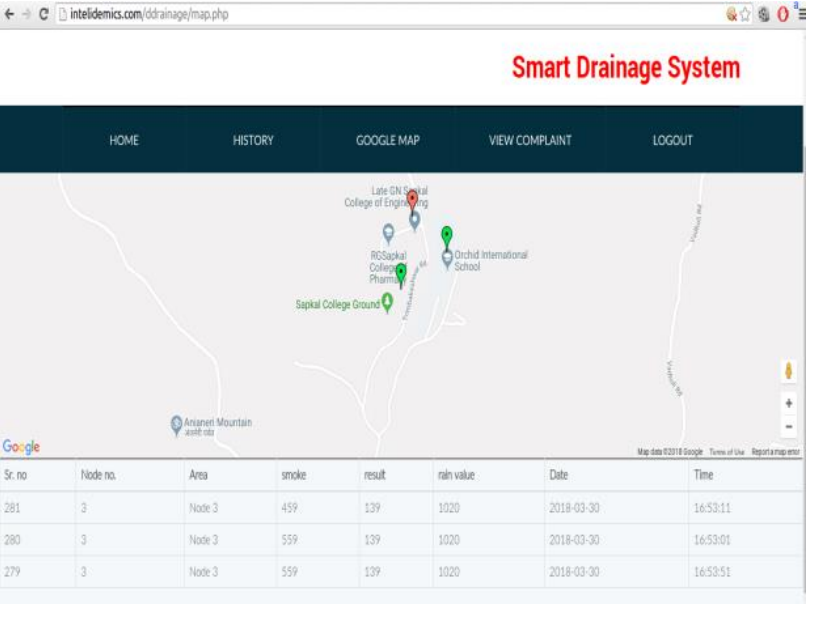
\includegraphics[width=0.85\textwidth]{Images/sonawane_dashboard.png}
    \caption{Web dashboard of the Smart Real-Time Drainage Monitoring System showing node readings and alert statuses \citep{sonawane2018}}
    \label{fig:sonawane_dashboard}
 \end{figure}


 \begin{figure}[h]
     \centering
     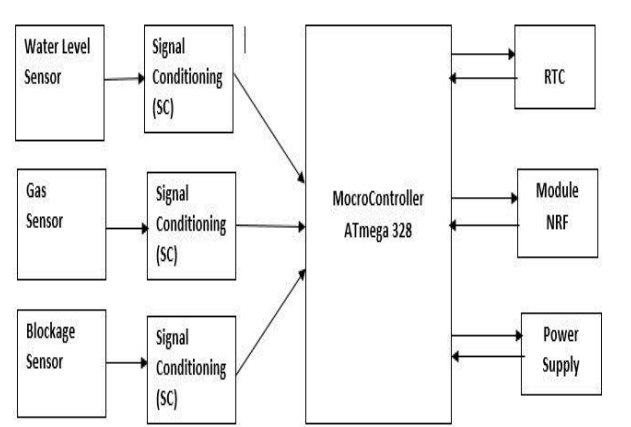
\includegraphics[width=0.85\textwidth]{Images/sonawane_blockdiagram.png}
     \caption{Block diagram of the sensor node hardware architecture \citep{sonawane2018}}
     \label{fig:sonawane_blockdiagram}
 \end{figure}
\clearpage
The system demonstrated the feasibility of using distributed IoT sensor nodes to monitor drainage conditions in real time, including gas detection, water level monitoring, and blockage detection across multiple connected manholes. The use of node-to-node communication via NRF modules provided a practical approach to data relay across drainage networks without requiring direct connectivity at every node, and the web-based dashboard provided a centralised view of drainage conditions across all monitored nodes.

However, the system did not incorporate any machine learning or predictive analytics capability, meaning it could only report current sensor readings rather than predict future drainage states or flood risk. The communication architecture relied on NRF modules with a reported range of only ten feet, significantly limiting the practical deployment distance between nodes. Additionally, the system was tested only in a workshop and limited open-air environments rather than within actual drainage channels, raising questions about sensor durability under real drainage conditions \citep{sonawane2018}.

\subsubsection{IoT-Based Smart Drainage System for Flood Management in Mogadishu, Somalia}

\citet{nageye2025} developed an IoT-based smart drainage system tailored to the flooding challenges of Mogadishu, Somalia, a context that shares several characteristics with Nairobi's urban drainage environment including inadequate infrastructure, reactive management practices, and recurrent flooding during heavy rainfall seasons. The system targeted municipal authorities and emergency management stakeholders who required real-time visibility into drainage conditions across the city's network of drainage collection points.

The system integrated ultrasonic HC-SR04 sensors for water level monitoring and YF-S201 Hall effect flow meters for measuring water flow rates at critical drainage collection points. Sensor data was transmitted via SIM800L GSM GPRS modules to an AWS cloud platform where it was processed and visualised through a web application built using Python Django. The system also incorporated solar-powered DC submersible water pumps that were automatically activated when water levels exceeded a predefined threshold, physically transporting excess water through HDPE pipes to the ocean to actively mitigate flooding rather than merely detecting it \citep{nageye2025}. Field testing across three high-risk flood zones in Mogadishu over six months demonstrated that the HC-SR04 ultrasonic sensors achieved a 98.7\% accuracy rate compared to manual water level measurements, with an average system response time of 3.2 seconds from threshold detection to alert generation.


 \begin{figure}[h]
     \centering
     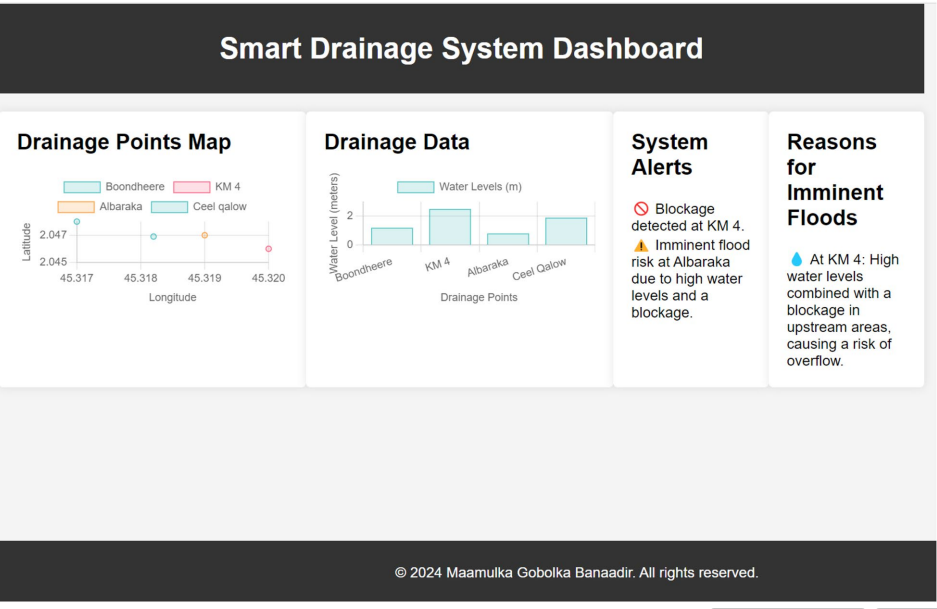
\includegraphics[width=0.85\textwidth]{Images/nageye_dashboard.png}
     \caption{Smart Drainage System Dashboard showing real-time water levels, system alerts, and reasons for imminent flooding \citep{nageye2025}}
     \label{fig:nageye_dashboard}
 \end{figure}


 \begin{figure}[h]
     \centering
     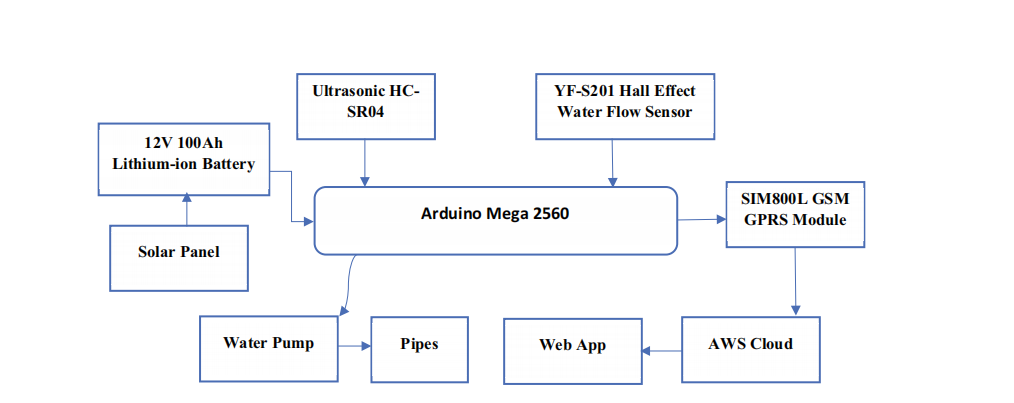
\includegraphics[width=0.85\textwidth]{Images/nageye_architecture.png}
     \caption{Proposed system architecture of the IoT-based smart drainage system for Mogadishu \citep{nageye2025}}
     \label{fig:nageye_architecture}
 \end{figure}
\clearpage
The system demonstrated a highly practical and deployable architecture for real-time drainage monitoring in a developing urban context, with validated sensor accuracy and system reliability under real-world field conditions. The professional web dashboard provided decision-makers with not only current sensor readings but also specific reasons for imminent flooding at each drainage location, significantly improving the actionability of the system's outputs. The use of solar power and battery backup addressed the power supply challenges commonly faced in resource-constrained environments.

Despite these strengths, the system did not incorporate machine learning or predictive analytics, and the authors explicitly acknowledge that the lack of labelled data precluded the development of predictive models \citep{nageye2025}. The system was therefore capable of detecting current flood risks based on threshold comparisons but could not predict future water level trends or generate early warnings before critical thresholds were reached. Additionally, the system did not include gas monitoring for harmful gases within drainage channels, leaving a significant public health dimension unaddressed.

\subsubsection{IoT-Based Flood Monitoring and Control System}

\citet{kumar2025} presented an IoT-based flood monitoring and control system designed to provide real-time flood detection, early warning generation, and automated flood control in both urban and rural flood-prone areas. The system targeted local authorities, emergency services, and residents in flood-prone zones who required timely alerts and automated responses to rising water levels. The system was explicitly designed to operate with minimal human intervention and without complex artificial intelligence algorithms, focusing instead on threshold-based decision logic to trigger alerts and automated control mechanisms such as floodgate activation \citep{kumar2025}.

The system utilised a network of water level sensors, rainfall gauges, soil moisture sensors, and temperature and humidity sensors connected to an Arduino UNO microcontroller interfaced with an ESP8266 Wi-Fi module for cloud connectivity. Sensor data was continuously compared against predefined threshold values, with the system generating SMS alerts and activating automated control responses when thresholds were exceeded. The system classified water levels into four zones: normal, yellow caution zone, red alert zone, and high alert flood zone, with corresponding alert messages and automated actions triggered at each level.


 \begin{figure}[h]
     \centering
     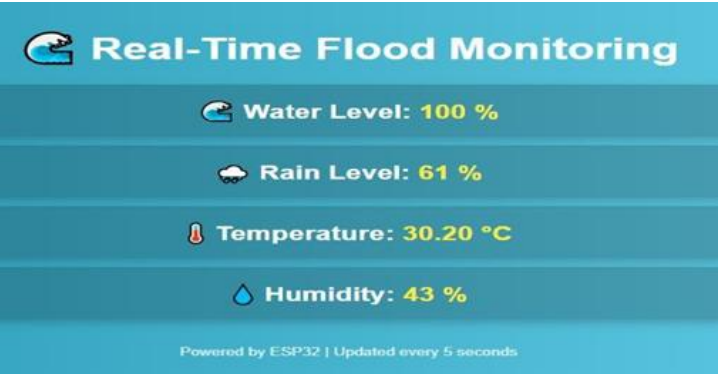
\includegraphics[width=0.75\textwidth]{Images/kumar_dashboard.png}
     \caption{Real-time flood monitoring dashboard displaying water level, rain level, temperature, and humidity readings \citep{kumar2025}}
     \label{fig:kumar_dashboard}
 \end{figure}


 \begin{figure}[h]
     \centering
     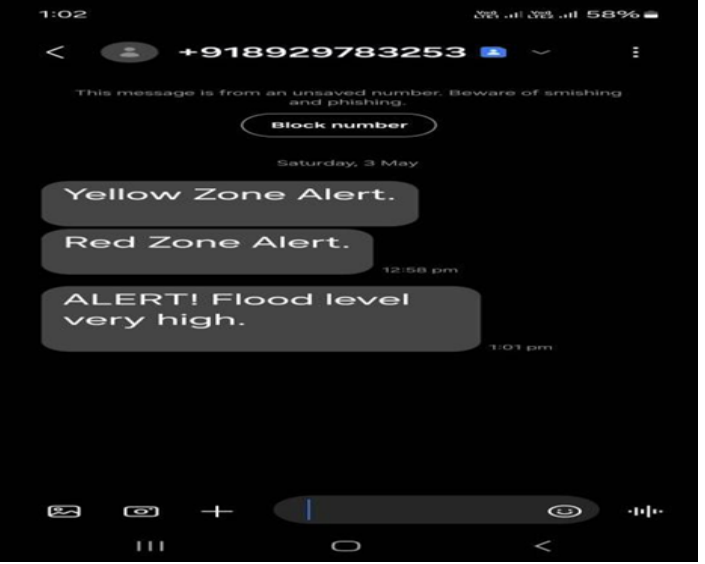
\includegraphics[width=0.5\textwidth]{Images/kumar_sms.png}
     \caption{SMS alert notifications generated by the flood monitoring system across alert zones \citep{kumar2025}}
     \label{fig:kumar_sms}
 \end{figure}

\clearpage
The system demonstrated a practical and cost-effective architecture for real-time flood monitoring using widely available and affordable components. The four-zone water level classification system provided a clear and actionable escalation framework that could be readily understood and acted upon by both authorities and residents. The automated control mechanisms including floodgate activation represented a meaningful step beyond passive monitoring toward active flood mitigation.

However, the system deliberately excluded machine learning and artificial intelligence techniques, relying entirely on static threshold comparisons that cannot adapt to changing drainage conditions or learn from historical sensor data patterns. This limits the system's ability to generate predictive early warnings before water levels reach critical thresholds. The system also did not incorporate flow rate monitoring, blockage detection, or gas sensing capabilities, making it unsuitable as a comprehensive drainage management solution \citep{kumar2025}.

\subsubsection{Machine Learning Implementations for Flood Prediction and Anomaly Detection}

The integration of machine learning into flood monitoring and prediction systems has emerged as a significant area of research, offering capabilities that go beyond the threshold-based detection approaches of basic IoT systems. This section reviews three key machine learning studies relevant to the proposed multi-model pipeline incorporating anomaly detection, Random Forest classification, and LSTM-based prediction.

The foundation of the proposed machine learning pipeline is an anomaly detection component that continuously monitors incoming sensor readings and flags significant deviations from established baseline drainage conditions. \citet{sathiyamoorthy2025} emphasise that real-time data integration is a critical component of effective flood management systems, enabling response to environmental changes as they occur rather than after they have escalated (p.~2). The technical basis for using flow rate differentials as a blockage detection mechanism is further supported by \citet{ramesh2026}, who deploy flow rate sensors alongside water level sensors at multiple drainage monitoring nodes and use the deviation in flow readings between adjacent nodes as a primary feature in a blockage prediction model. Their system achieves a false alarm rate below 10\% compared to 15 to 30\% for static threshold-based systems, demonstrating that flow-based differential analysis is a more reliable approach to blockage detection than water level thresholds alone. \citet{nagarajan2025} similarly demonstrate that rising water level deviations detected between monitoring points serve as reliable indicators of blockage events within drainage pipelines, providing further support for the flow differential approach adopted in the proposed system 

Random Forest classification is employed in the second stage of the proposed pipeline to classify the current state of the drainage system as Normal, Blockage Risk, or Flood Risk based on real-time sensor readings and the anomaly flag generated in the first stage. \citet{sathiyamoorthy2025} describe Random Forest as a technique that works well with predicting long-term data and data containing noise and missing values, making it well suited for sensor data collected in harsh drainage environments where readings may be affected by physical debris, moisture, and chemical contamination. In their comparative evaluation of flood prediction algorithms, Random Forest achieved an accuracy of 91.4\% with a precision of 90.2\% and recall of 92.5\%, demonstrating strong performance in classifying flood-related conditions from multi-source environmental data. Importantly, Random Forest also demonstrated the lowest computational resource requirements among the models tested, with an average processing time of 12 milliseconds and CPU usage of 45\%, making it practical for deployment in resource-constrained embedded system environments.

The third stage of the proposed pipeline employs a Long Short-Term Memory network to analyse historical sensor data trends and predict future water levels, estimating the time remaining before critical flood thresholds are reached. \citet{bao2025} demonstrate the application of LSTM networks for water depth prediction at multiple control points, showing that LSTM models trained on observed historical data can achieve Nash-Sutcliffe Efficiency values consistently above 0.98 and RMSE values ranging from 0.26 to 0.29 metres across multiple lead times, and that LSTM-based predictions could be generated for lead times of up to six hours, providing valuable advance warning of developing flood conditions. \citet{hiroi2016} similarly demonstrate that LSTM-based prediction trained on location-specific historical water level and rainfall data can detect complex water flow flooding five minutes earlier than actual water rising occurs, with a Root Mean Square Error of 2.8 centimetres under localised heavy rain conditions. \citet{banupriya2025} further support the use of LSTM networks for sequential sensor data analysis, noting that LSTM networks extract temporal dependencies and trends in rainfall, water levels, and soil displacement, and that combining LSTM with classification models produces more robust and accurate disaster prediction outcomes than using either approach in isolation.

\clearpage
\subsection{Gaps in Existing Systems and Machine Learning Implementations}

The review of existing drainage monitoring systems and machine learning implementations in Section 2.4 reveals several significant gaps that the proposed smart drainage monitoring and flood prediction system seeks to address.

The most fundamental gap across all three reviewed IoT systems is the absence of machine learning and predictive analytics capability. \citet{sonawane2018}, \citet{nageye2025}, and \citet{kumar2025} all present systems that rely on threshold-based comparisons of current sensor readings to predefined static values. While this approach can detect when conditions have already deteriorated to a dangerous level, it cannot predict that deterioration before it occurs, leaving authorities with little or no lead time for preventive action. \citet{nageye2025} explicitly acknowledge this gap, noting that the lack of labelled data precluded the development of predictive models in their system and recommending that future research explore the inclusion of predictive analytics.

A second significant gap is the absence of harmful gas monitoring in the flood monitoring and IoT drainage systems reviewed. Only \citet{sonawane2018} incorporated gas sensing into their system design, and even then the system did not monitor ammonia, which is also generated through decomposition of organic waste in drainage channels. Neither the Somalia system by \citet{nageye2025} nor the flood monitoring system by \citet{kumar2025} incorporated any form of gas detection, meaning that the public health and occupational safety dimension of drainage management remains entirely unaddressed in these systems.

A third gap relates to the integration of multi-stage machine learning pipelines that combine anomaly detection, classification, and prediction into a single cohesive system. The machine learning studies reviewed by \citet{sathiyamoorthy2025}, \citet{bao2025}, and \citet{banupriya2025} each address individual components of the prediction problem in isolation. None of the reviewed studies presents a system that combines anomaly detection as an initial trigger, Random Forest classification for real-time drainage state assessment, and LSTM-based prediction for future water level forecasting within a single integrated pipeline applied to urban drainage sensor data. Research by \citet{gandhimathinathan2024} demonstrates that combining LSTM-based feature extraction with Isolation Forest anomaly scoring produces superior detection performance compared to either technique applied independently, achieving an overall accuracy of 98.2\% on industrial sensor data. Similarly, \citet{yogarajan2025} show that hybrid anomaly detection frameworks combining Isolation Forest with density-based clustering consistently outperform single-model approaches across multiple IoT sensor datasets, achieving accuracies above 97\% on environmental and meteorological sensor streams. These findings support the design decision in the proposed system to pipeline anomaly detection, Random Forest classification, and LSTM prediction as complementary stages rather than treating any single technique as a complete solution.

Finally, none of the reviewed systems were designed or evaluated within the specific context of Kenyan urban drainage environments, where the combination of rapid urbanisation, informal settlements, solid waste accumulation in drainage channels, and inadequate stormwater infrastructure creates a unique and compounded set of drainage management challenges. The proposed system therefore seeks to address these gaps by developing a prototype that integrates real-time sensor monitoring, harmful gas detection, blockage identification, and a three-stage machine learning pipeline within the specific operational context of urban drainage management in Nairobi, Kenya.
\clearpage
\subsection{Conceptual Framework}

The conceptual framework presented in this section provides a visual and descriptive representation of the expected inputs, processes, outputs, and feedback mechanisms of the proposed smart drainage monitoring and flood prediction system. The framework illustrates how the system's components interact to transform raw sensor data into actionable information for county authorities and disaster management agencies.

 \begin{figure}[h]
     \centering
     \includegraphics[width=\textwidth]{Images/conceptual_framework.png}
     \caption{Conceptual Framework of the Smart Drainage Monitoring and Flood Prediction System}
     \label{fig:conceptual_framework}
 \end{figure}

\clearpage
The input layer of the conceptual framework represents the physical data collection component of the system. Distributed sensor nodes equipped with water level sensors, flow rate sensors, and gas sensors continuously collect measurements from within urban drainage channels. These readings are transmitted in real time to the centralised processing platform using the MQTT communication protocol, which provides lightweight and reliable data transmission suited to the constrained network environments typical of urban drainage deployments.

The system processing layer represents the analytical core of the proposed system and operates in three sequential stages. In the first stage, an anomaly detection algorithm continuously monitors incoming sensor readings against established baseline conditions and flags any significant deviations as indicators requiring further analysis. In the second stage, a Random Forest classification model evaluates the current sensor readings alongside the anomaly flag to classify the drainage state as Normal, Blockage Risk, or Flood Risk, providing a clear and immediately actionable status update. In the third stage, an LSTM model analyses the historical trend of sensor readings leading up to the current moment to predict future water levels and estimate the time remaining before critical flood thresholds are reached.

The output layer represents the information products delivered to system users through a web-based monitoring dashboard. Outputs include real-time drainage condition displays, early flood warning alerts with estimated time to critical threshold, blockage location alerts identifying the section of drainage channel where a flow rate discrepancy has been detected between two consecutive monitoring nodes, gas hazard alerts when harmful gas concentrations exceed safe thresholds, and historical analytical reports that support longer-term drainage planning and maintenance scheduling.

The actors in this framework are county authorities and disaster management agencies, who receive the system's outputs through the web-based dashboard and alert notifications. These actors are responsible for interpreting the system's alerts and reports, deploying maintenance teams to identified blockage locations, issuing public warnings when flood risk alerts are generated, and responding to gas hazard alerts by dispatching appropriate safety personnel. The feedback loop from these actors back to the system represents the maintenance actions and calibration updates that result from field investigations, which in turn improve the accuracy of the system's baseline models and classification thresholds over time.

\section{Development Methodology}

\subsection{Introduction}

This chapter discusses the software development methodology and the different aspects of the system analysis and design for the smart drainage monitoring and flood prediction system. The chapter begins by outlining the research paradigm adopted for the project, including the approaches that will be used for data acquisition, data preprocessing, model training, model validation and testing, and model evaluation metrics. It then defines and justifies the Agile software development methodology selected for the project, describing each phase of the methodology in the context of the system being developed. The chapter further presents the system analysis and design through detailed descriptions of the use case diagram, class diagram, entity relationship diagram, database schema, system architecture, and wireframes. Additionally, the chapter identifies the development tools and techniques that will be used in building the system and concludes by describing the modules and deliverables that will be produced at the end of the development process.

\subsection{Research Paradigm}

This project adopts a mixed research paradigm that integrates
exploratory and experimental approaches operating across three
distinct but complementary methodological layers. The first
layer is the overarching research paradigm which governs the
entire study. The second layer is the Cross Industry Standard
Process for Data Mining (CRISP-DM), which provides a structured
methodology for the machine learning pipeline development. The
third layer is Agile Scrum, which governs the software and
hardware development process. Together these three layers
provide a comprehensive and academically grounded framework
for managing the different components of this project.

The exploratory component of the research paradigm involves
the review of existing urban drainage monitoring systems and
flood management practices in Kenya to identify the specific
challenges and gaps that the proposed system seeks to address,
as documented in Chapter 2. This exploratory phase informs the
design decisions made throughout the system development process
and ensures that the proposed solution is grounded in a thorough
understanding of the problem environment.

The experimental component involves the design, development,
and empirical evaluation of the proposed smart drainage
monitoring and flood prediction system. Sensor nodes will be
physically constructed and tested within a controlled prototype
environment to generate sensor data, and the multi-model
machine learning pipeline will be trained and evaluated against
measurable performance metrics. The experimental nature of this
project aligns with the approach commonly adopted in artificial
intelligence and IoT system development research, where a
functional prototype is built, tested under realistic
conditions, and evaluated based on quantifiable outcomes such
as prediction accuracy, alert response time, and sensor
reliability \citep{sathiyamoorthy2025}.

In line with the experimental research paradigm, this study is
guided by the following research hypothesis:

\textit{A multi-model machine learning pipeline incorporating
Isolation Forest anomaly detection, Random Forest drainage
state classification, and Long Short-Term Memory flood risk
prediction, trained on publicly available drainage and flood
datasets, will achieve a minimum classification accuracy of
80\% in identifying drainage states and generate flood risk
predictions with a minimum lead time of five minutes within
a controlled prototype environment.}

This hypothesis is directly testable using the evaluation
metrics defined in Section 3.2.8 and provides a measurable
criterion against which the experimental outcomes of the
prototype testing phase will be assessed.

\subsubsection{Data Acquisition}

Data acquisition refers to the process of collecting raw data
from real-world sources for use in training, validating, and
evaluating machine learning models \citep{bao2025}. Since no
organisational drainage data is available for this project,
all training data will be sourced from publicly available
academic and open-data repositories. The datasets are
organised by the model they primarily support within the
three-stage machine learning pipeline.

For the Isolation Forest anomaly detection model, training
requires continuous multivariate sensor readings representing
normal operating conditions. Two datasets from the UCI
Machine Learning Repository will be used for this purpose.
\citet{gas_sensor_array_drift_dataset_224} provide the Gas
Sensor Array Drift Dataset, a multivariate time-series dataset
containing continuous readings from 16 chemical sensors
exposed to six different gases over 36 months, providing
realistic gas concentration patterns for establishing
baseline normal gas readings. \citet{twin_gas_sensor_arrays_361}
provide the Twin Gas Sensor Arrays dataset containing sensor
readings from two co-located gas sensor arrays under varying
environmental conditions. These will be supplemented by two
Kaggle datasets: the IoT T-Sensor Dataset for Anomaly
Detection \citep{iot_tsensor_kaggle}, which contains labelled
normal and anomalous IoT sensor readings; and the Sensor Data
dataset \citep{sensor_data_joshi}, which provides synthetic
sensor readings covering a range of operational states.

For the Random Forest classification model, training requires
a labelled dataset where drainage conditions are categorised
as Normal, Blockage Risk, or Flood Risk. Three datasets will
be used. The Flood Prediction Dataset from Kaggle
\citep{flood_prediction_kaggle} provides labelled flood and
non-flood condition records. The Urban Flood Risk Data: Global
City Analysis 2025 from Kaggle \citep{urban_flood_risk_kaggle}
provides flood risk classifications across global urban areas
including comparable developing-world drainage contexts. The
flood quality monitoring dataset from Zenodo
\citep{zenodo_flood_quality} provides water quality and flood
monitoring sensor records supporting the labelling of all
three drainage states.

For the LSTM flood prediction model, training requires long
sequential time-series data recorded at regular intervals
covering both normal and flood conditions. The Global Runoff
Data Centre provides historical river discharge time-series
data for East African river systems \citep{grdc_data}, while
the GloFAS ERA5 river discharge reanalysis dataset accessed
through the Copernicus Climate Data Store \citep{glofas_era5}
provides hourly water level reanalysis data for Kenya going
back decades. \citet{zhou2025} note that real-world IoT data
is often limited by noise, imbalance, and insufficient
coverage of rare or extreme conditions, and that supplementary
data generation strategies are necessary to produce training
datasets that adequately represent the range of conditions a
deployed model will encounter. \citet{anderson2014} similarly
demonstrate that synthetic data generation techniques can
produce datasets that preserve the statistical and structural
characteristics of original IoT sensor data, enabling
effective model training where direct data collection is
constrained. In addition to the above sources, sensor data
will be generated during the prototype testing phase within
a controlled laboratory environment where water levels and
flow conditions can be manually adjusted to simulate Normal,
Blockage Risk, and Flood Risk drainage states.

\subsubsection{CRISP-DM Machine Learning Methodology}

The Cross Industry Standard Process for Data Mining (CRISP-DM)
is an internationally recognised iterative methodology for
structuring data science and machine learning projects across
six sequential phases: Business Understanding, Data
Understanding, Data Preparation, Modelling, Evaluation, and
Deployment \citep{wirth2000}. CRISP-DM is adopted in this
project to provide a structured process for managing the
development of the three machine learning models, each of
which has distinct data requirements, training approaches,
and evaluation criteria.

In the Business Understanding phase, the objectives of each
model are defined in terms of the drainage problem. The
Isolation Forest is required to detect significant deviations
from baseline sensor readings that may indicate developing
blockage or flood conditions. The Random Forest is required to
classify incoming sensor readings into one of three drainage
states: Normal, Blockage Risk, or Flood Risk. The LSTM is
required to predict future water levels with a minimum lead
time of five minutes.

In the Data Understanding phase, each dataset sourced from
the UCI Machine Learning Repository, Kaggle, the Global
Runoff Data Centre, and Zenodo is examined for structure,
completeness, temporal regularity, and suitability for each
model. Missing values, outliers, and class imbalances are
identified at this stage for each dataset independently
before preprocessing begins.

The Data Preparation phase covers the preprocessing activities
described in Section 3.2.3, including cleaning, normalisation,
feature engineering, labelling for the Random Forest, and
sliding window sequence construction for the LSTM. Each model
receives a separately prepared dataset tailored to its
specific input requirements. The Modelling phase corresponds to Section 3.2.6, where each model is trained and hyperparameters are tuned using cross-validation. The
Evaluation phase corresponds to Section 3.2.8, where each
model is assessed against the defined performance metrics
before being accepted into the pipeline. A model that does
not meet the minimum performance threshold is returned to
the Modelling or Data Preparation phase for further
refinement. The Deployment phase corresponds to Section 3.6,
where the validated models are integrated into the backend
application and connected to the real-time MQTT data
ingestion pipeline.

\subsubsection{Data Preprocessing}

Data preprocessing refers to the set of transformations applied to raw collected data to prepare it for use in machine learning model training and evaluation. Raw sensor data collected from drainage environments is likely to contain missing values caused by connectivity interruptions, outlier readings caused by sensor malfunctions or physical debris, and inconsistencies between data collected from different sensor types and sources. These issues must be addressed before the data can be used for training to avoid introducing noise or bias into the machine learning models.

Preprocessing activities will include data cleaning to handle missing values through interpolation or removal, outlier detection and filtering to remove anomalous sensor readings that fall outside physically plausible ranges, normalisation of sensor readings to a consistent scale to ensure that no single sensor type dominates the model training process, and feature engineering to derive additional meaningful variables from the raw readings, such as rate-of-change in water level over time and flow rate differentials between adjacent monitoring nodes. The preprocessed dataset will be split into training, validation, and testing subsets following an 80-10-10 ratio to ensure that the model is evaluated on data it has not previously encountered during training.

\subsubsection{Evaluation Plan}
\label{sec:evaluation-plan}
 
Evaluating the machine learning pipeline requires data whose ground truth is known with certainty, which publicly sourced datasets cannot provide for this system's specific sensors and drainage context (Section~3.2.1). Evaluation data is therefore generated directly from the physical prototype described in Section~3.4, under two categories of controlled conditions.
 
The first category is a \textbf{Normal-condition baseline period}, in which the prototype is run continuously over a period during which it can be left unattended without requiring intervention -- in practice, approximately 48 hours, with the channel unobstructed and no artificial inflow beyond ordinary operation. Sensor readings collected during this period establish the range of water level, flow rate, and gas concentration values considered normal, and this baseline is the sole data source used to train the Isolation Forest anomaly detector (Section~3.2.6).
 
The second category is a set of \textbf{staged trials}, in which specific drainage conditions are deliberately created on the prototype by manually obstructing the channel and manually adjusting the rate of water added to the channel. Because each trial's condition is set by the experimenter, the correct label for that trial is known with certainty at the time it is run, rather than inferred afterward from the readings themselves. These staged trials, together with the criteria used to define each condition, are detailed in Section~3.2.5. Staged trial data is kept entirely separate from the Normal-condition baseline used for training: it is held out and used only to evaluate the trained models, following the training/evaluation separation illustrated in Figure~\ref{fig:threshold-split} and described in Section~3.2.6. The specific metrics computed from this evaluation data for each of the three models are detailed in Section~3.2.8.
 
\subsubsection{Labelling Protocol for Drainage State Classification}
\label{sec:labelling-protocol}
 
The Random Forest classification model is a supervised algorithm and therefore requires a labelled training example for every drainage state it is intended to recognise. Rather than inferring these labels from the sensor readings after the fact -- which would risk the model simply reproducing whatever threshold rule was used to generate the labels -- each label is assigned by the experimenter at the time a condition is staged on the physical prototype, according to the following protocol. The two sensor nodes are positioned along the channel with a section between them that can be manually obstructed -- either by hand or by repositioning a length of pipe -- so that restricting flow at that point produces a measurable flow differential between the upstream and downstream node, consistent with the blockage detection approach defined in Section~1.5.1.
 
\begin{itemize}
    \item \textbf{Normal:} Water level and flow rate at both nodes remain within the range established during the Normal-condition baseline period (Section~\ref{sec:evaluation-plan}), and flow rate readings at the upstream and downstream nodes remain consistent with one another. No gas concentration exceeds its baseline range, and no manual obstruction is applied.
    \item \textbf{Blockage Risk:} The channel between the two nodes is manually obstructed -- by hand or by repositioning a section of pipe -- to a degree kept as consistent as possible across trials. This produces a measurable and sustained drop in flow rate at the downstream node relative to the upstream node -- the same node-to-node flow differential described in Section~1.5.1 -- while water level rises above its baseline range at the upstream node. Every reading collected for the duration of this obstruction is labelled Blockage Risk.
    \item \textbf{Flood Risk:} Inflow to the prototype is increased by manually adding water to the channel at a faster rate than normal (for example, using a jug or watering can) while the channel remains obstructed, producing a rate of water level rise that exceeds a fixed threshold calibrated during the baseline period. Every reading collected for the duration of this condition is labelled Flood Risk.
\end{itemize}
 
\noindent Because the condition being staged is known and controlled by the experimenter at the moment each trial is run, labels are assigned with certainty rather than estimated, and the same staged trials serve as the held-out evaluation data described in Section~\ref{sec:evaluation-plan} once the model has been trained. This protocol also means the Blockage Risk label is grounded in the same flow-differential mechanism the system uses operationally to detect blockages (Section~1.5.1), rather than an independent or conflicting definition introduced solely for model training purposes. Because both the channel obstruction and the increased inflow are applied manually rather than through calibrated mechanical equipment, the degree of restriction and the rate of added water are kept as consistent as practicable across trials (for example, by marking a fixed pipe position or obstruction depth, and using a container of known volume to add water at a repeatable pace), and this reliance on manual staging is itself noted as a limitation in Section~1.5.2.

\subsubsection{Model Training}

Model training refers to the process of exposing a machine learning algorithm to a labelled training dataset so that it can learn the patterns and relationships within the data and use them to make predictions or classifications on new, unseen data. In this project, three machine learning models will be trained as part of the multi-model pipeline, each using a distinct mathematical formulation appropriate to its role in the system.

The exact data flow connecting the three stages is stated explicitly in Table~\ref{tab:pipeline-dataflow} and illustrated in Figure~\ref{fig:pipeline-dataflow}, to make clear that each stage's output is a necessary input to the next rather than three models applied independently to the same raw data.
 
\begin{table}[H]
\centering
\caption{Data flow through the three-stage machine learning pipeline}
\label{tab:pipeline-dataflow}
\begin{tabular}{|p{3.6cm}|p{5.7cm}|p{5.7cm}|}
\hline
\textbf{Stage} & \textbf{Input} & \textbf{Output} \\
\hline
1. Isolation Forest (Anomaly Detection) &
A single timestamped sensor reading vector: water level (cm), flow rate (lpm), and three gas concentrations (CH4, H2S, NH3 in ppm) &
An anomaly score (continuous value) and a binary anomaly flag \\
\hline
2. Random Forest (Drainage State Classification) &
The same sensor reading vector, with the Stage~1 anomaly flag appended as an additional feature &
A predicted class label: Normal, Blockage Risk, or Flood Risk \\
\hline
3. LSTM (Flood Risk Prediction) &
A sliding window of the last $N$ timestamped sensor readings, together with the sequence of Stage~2 class labels over that window &
A predicted water level/flow trajectory for the next $M$ minutes, and an estimated time-to-threshold \\
\hline
\end{tabular}
\end{table}
 
\begin{figure}[H]
    \centering
    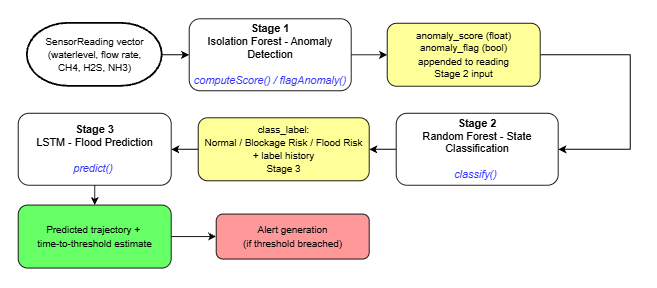
\includegraphics[width=\textwidth]{Images/ML_Pipeline_DataFlow_Diagram.png}
    \caption{Data flow between the three machine learning pipeline stages}
    \label{fig:pipeline-dataflow}
\end{figure}
 
\noindent Stage~1's output is not discarded after use -- it is passed forward as an input feature to Stage~2, and Stage~2's classification history forms part of the input sequence to Stage~3. The pipeline is therefore sequential and cumulative, as shown above, rather than three independent models applied separately to the same raw sensor data.

The anomaly detection component will be implemented using an Isolation Forest algorithm, which detects anomalies by isolating observations through random recursive partitioning of the feature space. For a given observation $x$, the anomaly score $AS(x)$ is defined as:

\begin{equation}
AS(x) = 2^{-\frac{E(h(x))}{c(n)}}
\end{equation}
\myequations{Isolation Forest Anomaly Score}

where $E(h(x))$ is the expected path length of observation $x$ across all isolation trees, $c(n) = 2H(n-1) - \frac{2(n-1)}{n}$ is the average path length of an unsuccessful search in a binary search tree, $H(i)$ is the harmonic number, and $n$ is the number of training samples \citep{salim2024}. Observations with anomaly scores approaching 1 are flagged as anomalies, while scores near 0.5 indicate normal observations. 

\paragraph{Training and Evaluation Data Separation}
The Isolation Forest anomaly detector is trained in a strictly unsupervised manner: it is fitted only on sensor readings collected during the 48-hour Normal-condition baseline period described in Section~\ref{sec:evaluation-plan}, without any label information attached to that data. No staged Blockage Risk or Flood Risk trial data is included in this training set.
 
Evaluation of the anomaly detector is a separate step, using a held-out set of labelled data consisting of the staged trials described in Section~\ref{sec:labelling-protocol}. Because these trials are labelled by construction -- the experimenter controls and records which condition was staged for each trial -- they provide ground truth against which the detector's flagging behaviour can be checked, without that labelled data ever having been used to train the detector itself. Figure~\ref{fig:threshold-split} illustrates this separation.
 
\begin{figure}[H]
    \centering
    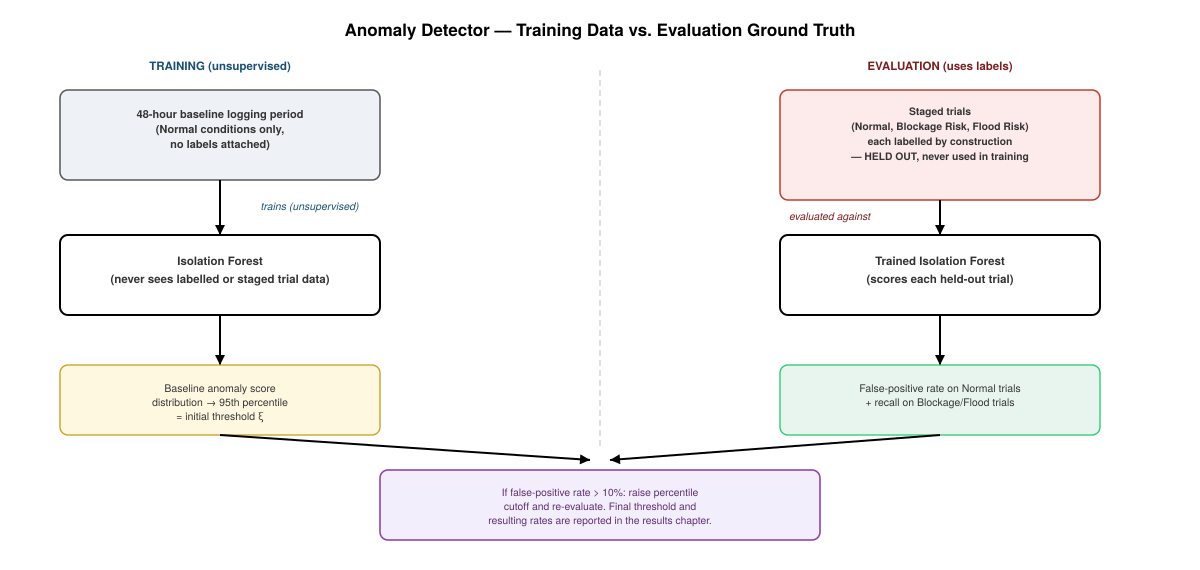
\includegraphics[width=\textwidth]{Images/Anomaly_Detector_Training_Evaluation_Split.png}
    \caption{Separation between unsupervised training data and labelled evaluation data for the anomaly detector}
    \label{fig:threshold-split}
\end{figure}
 
\paragraph{Anomaly Threshold Selection}
 
The anomaly score threshold $\xi$ is selected as follows: the 95th percentile of anomaly scores observed during the Normal-condition baseline period is used as the initial threshold. This threshold is then evaluated against the held-out staged trials; if the resulting false-positive rate (baseline-like readings incorrectly flagged as anomalous) exceeds 10\%, the percentile cutoff is raised and the threshold is re-evaluated. The final chosen threshold, together with the false-positive rate and recall it produces on the held-out staged trials, is reported in the results chapter.

The Random Forest classification model classifies the current drainage state as Normal, Blockage Risk, or Flood Risk by aggregating predictions from an ensemble of $T$ decision trees. For a given input vector $\mathbf{x}$ containing the current sensor readings and anomaly flag, each tree $t$ produces a class prediction $\hat{y}_t(\mathbf{x})$, and the final classification is determined by majority vote:

\begin{equation}
\hat{y}(\mathbf{x}) = \arg\max_{c} \sum_{t=1}^{T} \mathbf{1}[\hat{y}_t(\mathbf{x}) = c]
\end{equation}
\myequations{Random Forest Classification by Majority Vote}

where $c \in \{\text{Normal}, \text{Blockage Risk}, \text{Flood Risk}\}$ and $\mathbf{1}[\cdot]$ is the indicator function \citep{sathiyamoorthy2025}. Each tree is trained on a bootstrapped subset of the training data using randomly selected feature subsets at each split node, which reduces variance and improves generalisation on noisy sensor data.

The LSTM prediction model is a recurrent neural network architecture designed to learn temporal dependencies in sequential sensor data. The LSTM unit processes the input sequence $\mathbf{x}_t$ at each time step $t$ through four gating mechanisms. The forget gate $f_t$, input gate $i_t$, candidate cell state $\tilde{c}_t$, output gate $o_t$, cell state $c_t$, and hidden state $h_t$ are computed as follows:

\begin{equation}
f_t = \sigma(W_f \cdot [h_{t-1}, x_t] + b_f)
\end{equation}
\myequations{LSTM Forget Gate}

\begin{equation}
i_t = \sigma(W_i \cdot [h_{t-1}, x_t] + b_i)
\end{equation}
\myequations{LSTM Input Gate}

\begin{equation}
\tilde{c}_t = \tanh(W_c \cdot [h_{t-1}, x_t] + b_c)
\end{equation}
\myequations{LSTM Candidate Cell State}

\begin{equation}
c_t = f_t \odot c_{t-1} + i_t \odot \tilde{c}_t
\end{equation}
\myequations{LSTM Cell State Update}

\begin{equation}
o_t = \sigma(W_o \cdot [h_{t-1}, x_t] + b_o)
\end{equation}
\myequations{LSTM Output Gate}

\begin{equation}
h_t = o_t \odot \tanh(c_t)
\end{equation}
\myequations{LSTM Hidden State}

where $\sigma$ is the sigmoid activation function, $\tanh$ is the hyperbolic tangent activation function, $W_f, W_i, W_c, W_o$ are the weight matrices, $b_f, b_i, b_c, b_o$ are the bias vectors, and $\odot$ denotes element-wise multiplication \citep{bao2025}. The model will be trained using a sliding window of historical sensor readings as input and the water level at the next time step as the prediction target, with the Root Mean Square Error loss function used during backpropagation through time.

All three models will be trained using Python with the scikit-learn library for the Isolation Forest and Random Forest components and the TensorFlow and Keras libraries for the LSTM component. Hyperparameter tuning will be conducted for each model using cross-validation, and training progress will be monitored using the evaluation metrics defined in Section 3.2.8.

\subsubsection{Model Validation and Testing}

Model validation and testing refers to the process of evaluating a trained machine learning model's performance on data that was not used during the training phase, to assess how well the model generalises to new and unseen conditions. Validation will be conducted using the validation subset of the dataset during the training phase to guide hyperparameter selection and prevent overfitting. Final model testing will be conducted using the held-out testing subset to produce the performance metrics that will be reported as the system's evaluation results.

In addition to offline evaluation using the held-out test data, the trained models will be evaluated under simulated conditions within the controlled prototype testing environment. Sensor inputs representing normal, blockage risk, and flood risk drainage states will be manually configured and fed through the complete machine learning pipeline, and the system's classification and alert outputs will be assessed for correctness and timeliness against the expected outcomes for each simulated scenario. The minimum acceptable performance threshold for the prediction model has been set at 80\% accuracy, consistent with the objective defined in Section 1.3.1.

\subsubsection{Model Evaluation Metrics}

The performance of each model within the machine learning pipeline will be evaluated using a defined set of metrics appropriate to the type of task each model performs. For the anomaly detection component, evaluation will focus on the recall rate, which measures the proportion of true anomalies correctly identified, and the false alarm rate, which measures the proportion of normal readings incorrectly flagged as anomalies. A high recall with a low false alarm rate is the target outcome, consistent with the performance achieved by \citet{salim2024} who report a recall of 0.9977 and a false alarm rate of 0.0003 using Extended Isolation Forest on industrial IoT sensor data.

For the Random Forest classification model, evaluation will use accuracy, precision, recall, and F1-score calculated across the three drainage state classes of Normal, Blockage Risk, and Flood Risk. A minimum accuracy threshold of 80\% has been set for this component, with F1-score used as the primary metric to account for potential class imbalance in the training dataset. \citet{sathiyamoorthy2025} report Random Forest achieving 91.4\% accuracy and an F1-score of 91.3\% on a comparable multi-class flood risk classification task, providing a benchmark for the expected performance range.

For the LSTM prediction model, evaluation centres on a direct lead-time experiment rather than error metrics alone, since RMSE and MAE describe average prediction error but do not by themselves establish whether a usable early warning was given in time.
 
The prediction horizon is fixed at five minutes: the LSTM is trained to predict water level $M = 5$ minutes ahead of the current reading. For each staged Flood Risk trial conducted on the physical prototype (Section~\ref{sec:labelling-protocol}), the exact timestamp at which water level first crosses the defined flood threshold is recorded as the trial's true onset time, $T_{onset}$. The model's prediction made at $T_{onset} - 5\text{min}$ is then checked: a trial counts as a successful early warning if the model correctly flags an approaching Flood Risk condition at or before this point. Figure~\ref{fig:leadtime-eval} illustrates this procedure for a single trial.
 
\begin{figure}[H]
    \centering
    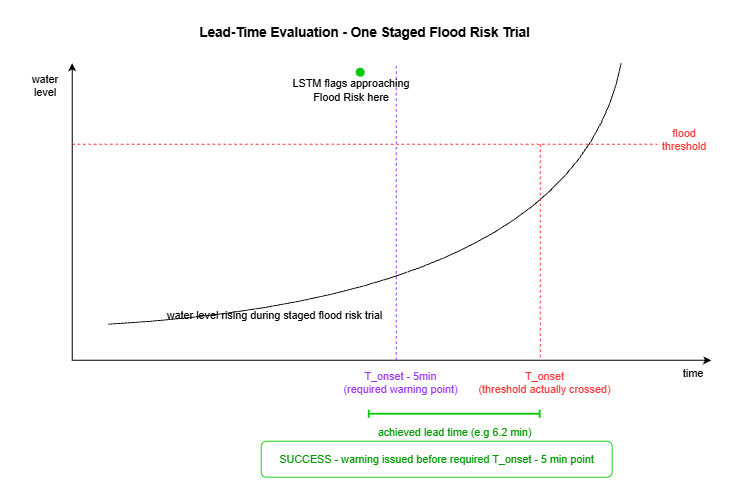
\includegraphics[width=\textwidth]{Images/LeadTime_Evaluation_Diagram.png}
    \caption{Lead-time evaluation procedure for a single staged Flood Risk trial}
    \label{fig:leadtime-eval}
\end{figure}
 
This procedure is repeated across multiple staged Flood Risk trials to produce a \textbf{lead-time success rate}: the proportion of trials in which the required five-minute warning was achieved. The \textbf{average achieved lead time} across successful trials is also reported (e.g., a mean of 6.2 minutes with a defined minimum and maximum), giving a more complete picture than a single pass/fail figure. In addition, the model is evaluated against staged Normal trials to establish a \textbf{false-positive rate}, since a model that frequently predicts flooding during genuinely normal conditions would not be a usable early-warning system regardless of its performance on flood trials.
 
Root Mean Square Error and Mean Absolute Error are still computed and reported as secondary metrics describing the LSTM's raw prediction accuracy, but are not treated as sufficient evidence of early-warning capability on their own. Published benchmark values from prior related work -- for example, \citet{jadhav2025} reporting an RMSE of 3.12 and an R-squared value of 0.88, and \citet{bao2025} reporting RMSE values between 0.26 and 0.29 metres across multiple lead times -- are treated strictly as reference points for comparable but not identical settings, and are not treated as expected or guaranteed outcomes for this system, which is evaluated on its own prototype under its own staged conditions.

\subsection{Software Development Methodology}

A software development methodology is a structured framework
that defines the processes, practices, and phases followed
when planning, building, testing, and delivering a software
system \citep{sommerville2016}. For this project, Agile Scrum
has been selected as the software development methodology for
the design and development of the smart drainage monitoring
and flood prediction system.

Agile Scrum is a specific Agile framework that organises
development work into fixed-length iterative cycles called
sprints, each of which produces a working and demonstrable
increment of the system. In the context of this project,
Mr. Ouma Kelvin acts as the Product Owner, responsible for
defining and prioritising system requirements and evaluating
each sprint increment through supervision sessions. The
student acts simultaneously as the Scrum Master, responsible
for managing the sprint process, and as the Development Team,
responsible for all design, implementation, and testing
activities. The project is organised into six sprints mapped
directly onto the Strathmore academic calendar: Sprint 1
covering requirements elicitation and system design during
April and May 2026; Sprint 2 covering sensor node
construction and MQTT setup in August and September 2026;
Sprint 3 covering data acquisition and preprocessing in
September 2026; Sprint 4 covering machine learning model
development in September and October 2026; Sprint 5
covering dashboard development and integration from October
to November 2026; and Sprint 6 covering testing, evaluation,
and documentation in November 2026. The suitability of Agile
Scrum for IoT system development is well established in
the literature. \citet{gouthaman2018} argue that Agile-based
software development is the most fitting process for managing
IoT systems due to the iterative hardware-software integration
challenges inherent in such projects, while \citet{jusoh2019}
find that 100\% of surveyed IoT development organisations
adopt Agile methodologies with Scrum being the most widely
used framework.

% -------------------------------------------------------
% INSERT FIGURE HERE
% Take a screenshot of the Agile methodology diagram
% generated in the chat.
% Save as agile_diagram.png in your images/ folder
% and uncomment the lines below.
% -------------------------------------------------------
% \begin{figure}[h]
%     \centering
%     \includegraphics[width=\textwidth]{agile_diagram}
%     \caption{Agile Software Development Methodology as Applied to the Smart Drainage Monitoring and Flood Prediction System}
%     \label{fig:agile_diagram}
% \end{figure}

\subsubsection{Requirements Elicitation}

Requirements elicitation is the first phase of the Agile methodology and involves identifying, gathering, and documenting the functional and non-functional requirements of the proposed system through engagement with relevant stakeholders. In this project, requirements elicitation will involve a review of existing drainage management practices and challenges within selected urban drainage environments in Nairobi, informed by the literature review conducted in Chapter 2. Functional requirements will include the system's ability to monitor water levels, flow rates, and harmful gas concentrations in real time, detect drainage blockages through flow rate differentials between adjacent sensor nodes, classify drainage states using a Random Forest model, predict future water levels using an LSTM model, and generate early warning alerts through a web-based dashboard. Non-functional requirements will include system reliability, sensor accuracy, alert response time, and dashboard accessibility for county authority users, disaster management agency users, and system administrators.

\subsubsection{System Design}

The system design phase involves translating the gathered requirements into detailed technical specifications and architectural descriptions that guide the development of the system. In this project, system design will encompass the design of the sensor node hardware architecture specifying the ESP32 microcontroller configuration and sensor connections, the design of the MQTT-based data transmission architecture connecting sensor nodes to the centralised platform, the design of the PostgreSQL database schema, the design of the web application architecture including the Flask or Django backend framework and dashboard interface layout, and the design of the machine learning pipeline specifying the inputs, outputs, and integration points of the anomaly detection, Random Forest, and LSTM components. The system design deliverables produced in this phase are presented in Section 3.4 of this chapter.

\subsubsection{Prototype Development}

The prototype development phase involves the physical construction and initial software implementation of the system based on the specifications produced during the system design phase. In this project, prototype development will involve assembling the distributed sensor nodes using ESP32 microcontrollers and connecting them to the selected sensors, implementing the MQTT communication protocol for data transmission between the nodes and the centralised platform, developing the initial version of the web-based monitoring dashboard, and implementing the basic data ingestion pipeline that collects and stores incoming sensor readings in the PostgreSQL database. The prototype produced in this phase will serve as the foundation for subsequent sensor integration and machine learning development sprints.

\subsubsection{Sensor Integration}

The sensor integration phase involves connecting and calibrating the physical sensor nodes within the controlled prototype testing environment and validating that sensor readings are accurately transmitted to and stored by the centralised monitoring platform. In this project, sensor integration will involve assembling a minimum of two sensor nodes using ESP32 microcontrollers and verifying that the ultrasonic water level sensors, flow rate sensors, and MQ-series gas sensors produce accurate and consistent readings under controlled conditions. Water level calibration will be conducted using a controlled water container where the depth is manually set and compared against sensor readings. Flow rate calibration will be conducted using a measured flow setup, and gas sensor readings will be validated against known reference concentration levels. Any sensor accuracy or connectivity issues identified during this phase will be resolved before the system proceeds to the machine learning development phase.

\subsubsection{Machine Learning Model Development}

The machine learning model development phase involves training, tuning, and integrating the three components of the proposed machine learning pipeline using the sensor data collected during the sensor integration phase, supplemented by the organisational and publicly available drainage datasets described in Section 3.2.1. The anomaly detection model will be trained first to establish baseline drainage conditions, followed by the Random Forest classification model trained on labelled drainage state data, and finally the LSTM prediction model trained on time-series sequences of historical sensor readings. Each model will be integrated into the web application backend and connected to the real-time data ingestion pipeline so that incoming sensor readings are automatically processed through the complete pipeline.

\subsubsection{Coding and Development}

The coding and development phase encompasses the full-stack implementation of the web-based monitoring dashboard and the supporting backend services that process sensor data, run the machine learning pipeline, and deliver outputs to system users. Development will follow Python conventions using Flask or Django for the backend application framework, with the machine learning models implemented using scikit-learn for the Isolation Forest and Random Forest components and TensorFlow with Keras for the LSTM component. The web-based dashboard will provide county authority users and disaster management agency users with real-time visualisations of drainage conditions, alert notifications, and historical analytical reports. The system administrator interface will provide tools for managing user accounts, configuring alert thresholds, and monitoring system health. The PostgreSQL database will be used for persistent storage of all sensor readings, alerts, user records, and report records.


\subsubsection{Testing and Deployment}

The testing and deployment phase involves systematically evaluating the completed system against the functional and non-functional requirements established during the requirements elicitation phase. Testing will include unit testing of individual system components, integration testing of the end-to-end data pipeline from sensor node to dashboard output, and prototype testing of the fully assembled system under simulated drainage conditions in a controlled environment. Performance metrics including prediction accuracy, alert response time, and sensor reading reliability will be recorded and evaluated against the minimum thresholds defined in the project objectives. Since the system is a prototype, deployment refers to the demonstration of the fully functional prototype in a controlled setting rather than installation within a live drainage infrastructure. Feedback gathered during prototype testing will be used to inform any final refinements to the system before the prototype is presented as the project deliverable.


\subsection{System Analysis and Design}

System design refers to the process of defining the architecture, components, interfaces, and data flows of a system to satisfy specified requirements. It translates the functional and non-functional requirements gathered during the requirements elicitation phase into a set of technical specifications and descriptions that guide the implementation of the system \citep{sommerville2016}.

\subsubsection{Use Case Diagram}

A use case diagram is a type of Unified Modelling Language behavioural diagram that illustrates the functional interactions between the actors of a system and the specific services or functions the system provides to those actors. Each actor represents a role played by a person or external system, and each use case represents a discrete functional requirement that the system must fulfil \citep{booch2005}.

The use case diagram for the smart drainage monitoring and flood prediction system identifies three actors. The County Authority User is a representative of the relevant county government office responsible for urban drainage management in Nairobi. This actor interacts with the system to view real-time sensor readings from all active monitoring nodes, receive flood warning alerts with estimated time to critical threshold, receive drainage blockage location alerts identifying the specific section of drainage channel affected, receive gas hazard alerts when harmful gas concentrations exceed safe thresholds, and generate historical analytical reports for drainage planning and maintenance scheduling. The Disaster Management Agency User is a representative of an emergency response organisation who requires timely information to coordinate flood response activities. This actor interacts with the system to receive flood risk alerts, view the current drainage state classification across all monitored nodes, and access historical incident reports to support post-event analysis. The System Administrator is responsible for managing the technical operation of the system and interacts with it to manage user accounts and role assignments for county authority and disaster management agency users, configure alert thresholds for water level, flow rate differential, and gas concentration sensors, monitor the operational health and connectivity status of all deployed sensor nodes, and manage sensor node registration and configuration settings. The use cases of viewing real-time sensor readings, receiving alerts, and accessing historical reports are shared between the County Authority User and the Disaster Management Agency User, while user account management, alert threshold configuration, and system health monitoring are restricted exclusively to the System Administrator role.

\subsubsection{Class Diagram}

A class diagram is a structural UML diagram that represents the classes within a system, their attributes and methods, and the relationships between them \citep{booch2005}. It provides a static view of the system's object-oriented architecture and serves as a blueprint for the software implementation.

The class diagram for the smart drainage monitoring and flood prediction system contains eight primary classes. The SensorNode class represents a physical monitoring node and holds attributes for node identifier, location name, latitude and longitude coordinates, and installation date. It provides methods for registering the node with the system and updating its operational status. The SensorReading class represents a single timestamped data record transmitted from a sensor node and holds attributes for reading identifier, the associated node identifier as a foreign key, timestamp, water level in centimetres, flow rate in litres per minute, and gas concentration readings for methane, hydrogen sulfide, and ammonia in parts per million. The AnomalyDetector class implements the Isolation Forest anomaly detection component and holds the trained model and the anomaly score threshold as attributes. It provides a method for computing the anomaly score of an incoming sensor reading and a method for flagging readings that exceed the threshold. The Drainage Classifier class implements the Random Forest classification model and holds the trained classifier and the list of drainage state labels as attributes. It provides a method that accepts a sensor reading and an anomaly flag as inputs and returns a drainage state classification of Normal, Blockage Risk, or Flood Risk. The FloodPredictor class implements the LSTM prediction model and holds the trained network, the input sequence length, and the prediction horizon as attributes. It provides a method that accepts a time-series sequence of recent sensor readings and returns a predicted future water level along with an estimated time to threshold. The Alert class represents a system-generated notification and holds attributes for alert identifier, the associated node identifier, alert type, severity level, descriptive message, timestamp, and the identifier of the user who acknowledged the alert. The User class manages system user accounts and holds attributes for user identifier, name, email address, hashed password, role, and account creation timestamp. It provides methods for authentication and role-based access verification. The Report class represents a generated analytical report and holds attributes for report identifier, the identifier of the generating user, the reporting period start and end dates, report type, and the file storage path. It provides a method for generating the report content based on sensor readings and alert records within the specified period.

The relationships between these classes are as follows. SensorNode has a one-to-many relationship with SensorReading, meaning one node generates many readings over time. SensorReading may be associated with many Alert records, representing a one-to-many relationship from reading to alerts. Alert has a many-to-one relationship with User through the acknowledgement field. User has a one-to-many relationship with Report, and Report has a many-to-many relationship with SensorNode through a report coverage association that records which nodes are included in each report.


\subsubsection{Entity Relationship Diagram}

An Entity Relationship Diagram is a data modelling tool that represents the entities within a system's data model, their attributes, and the relationships between them, providing a logical blueprint for the design of the database \citep{chen1976}.

The ERD for the smart drainage monitoring and flood prediction system contains five entities. The \texttt{SensorNode} entity represents a physical monitoring node and contains the attributes node identifier as the primary key, location name, latitude, longitude, and installation date. The \texttt{SensorReading} entity represents a single sensor data record and contains the attributes reading identifier as the primary key, node identifier as a foreign key referencing \texttt{SensorNode}, timestamp, water level, flow rate, methane concentration, hydrogen sulfide concentration, and ammonia concentration. The relationship between \texttt{SensorNode} and \texttt{SensorReading} is one-to-many, meaning one sensor node generates many sensor readings over time. The \texttt{Alert} entity represents a system-generated notification and contains the attributes alert identifier as the primary key, node identifier as a foreign key referencing \texttt{SensorNode}, alert type, severity, message, timestamp, and acknowledged by as a nullable foreign key referencing \texttt{User}. The relationship between \texttt{SensorNode} and \texttt{Alert} is one-to-many. The \texttt{User} entity represents a system account holder and contains the attributes user identifier as the primary key, name, email, password hash, role, and created at timestamp. The relationship between \texttt{User} and \texttt{Alert} through the acknowledged by field is many-to-one, meaning many alerts may be acknowledged by one user. The \texttt{Report} entity represents a generated analytical report and contains the attributes report identifier as the primary key, generated by as a foreign key referencing \texttt{User}, date from, date to, report type, and file path. The relationship between \texttt{User} and \texttt{Report} is one-to-many, meaning one user may generate many reports.

\subsubsection{Database Schema}

The database schema defines the physical structure of the system's PostgreSQL relational database. The schema implements six tables whose structure is detailed below.

\noindent\textbf{\texttt{sensor\_nodes}}
\vspace{4pt}
\begin{table}[H]
\centering
\caption{Structure of the \texttt{sensor\_nodes} table}
\begin{tabular}{|p{3.8cm}|p{2.8cm}|p{2cm}|p{5cm}|}
\hline
\multicolumn{4}{|l|}{\textbf{Table: sensor\_nodes}} \\
\hline
\textbf{Column} & \textbf{Data Type} & \textbf{Constraint} & \textbf{Description} \\
\hline
node\_id & SERIAL & PRIMARY KEY & Auto-incrementing unique identifier for each sensor node \\
\hline
location\_name & VARCHAR(100) & NOT NULL & Human-readable name of the drainage monitoring location \\
\hline
latitude & DECIMAL(9,6) & --- & Geographic latitude coordinate of the sensor node \\
\hline
longitude & DECIMAL(9,6) & --- & Geographic longitude coordinate of the sensor node \\
\hline
installation\_date & DATE & --- & Date on which the sensor node was installed \\
\hline
\end{tabular}
\end{table}

\begin{table}[H]
\centering
\caption{Structure of the \texttt{sensor\_readings} table}
\begin{tabular}{|p{3.8cm}|p{2.8cm}|p{2cm}|p{5cm}|}
\hline
\multicolumn{4}{|l|}{\textbf{Table: sensor\_readings}} \\
\hline
\textbf{Column} & \textbf{Data Type} & \textbf{Constraint} & \textbf{Description} \\
\hline
reading\_id & SERIAL & PRIMARY KEY & Auto-incrementing unique identifier for each sensor reading record \\
\hline
node\_id & INTEGER & FK $\rightarrow$ sensor\_nodes, CASCADE & Foreign key linking the reading to its originating sensor node \\
\hline
timestamp & TIMESTAMPTZ & DEFAULT NOW() & Date and time at which the sensor reading was recorded \\
\hline
water\_level\_cm & DECIMAL(6,2) & --- & Water level measured at the node in centimetres \\
\hline
flow\_rate\_lpm & DECIMAL(6,2) & --- & Water flow rate measured at the node in litres per minute \\
\hline
gas\_ch4\_ppm & DECIMAL(8,4) & --- & Methane (CH\textsubscript{4}) concentration in parts per million \\
\hline
gas\_h2s\_ppm & DECIMAL(8,4) & --- & Hydrogen sulfide (H\textsubscript{2}S) concentration in parts per million \\
\hline
gas\_nh3\_ppm & DECIMAL(8,4) & --- & Ammonia (NH\textsubscript{3}) concentration in parts per million \\
\hline
\end{tabular}
\end{table}

\noindent A composite index is created on node\_id and timestamp to support efficient time-series queries.

\begin{table}[H]
\centering
\caption{Structure of the \texttt{alerts} table}
\begin{tabular}{|p{3.8cm}|p{2.8cm}|p{2cm}|p{5cm}|}
\hline
\multicolumn{4}{|l|}{\textbf{Table: alerts}} \\
\hline
\textbf{Column} & \textbf{Data Type} & \textbf{Constraint} & \textbf{Description} \\
\hline
alert\_id & SERIAL & PRIMARY KEY & Auto-incrementing unique identifier for each alert record \\
\hline
node\_id & INTEGER & FK $\rightarrow$ sensor\_nodes & Foreign key identifying the sensor node that triggered the alert \\
\hline
alert\_type & VARCHAR(50) & --- & Category of alert: Flood Risk, Blockage, or Gas Hazard \\
\hline
severity & VARCHAR(20) & --- & Severity level of the alert: Low, Medium, or High \\
\hline
message & TEXT & --- & Descriptive text explaining the alert condition and recommended action \\
\hline
timestamp & TIMESTAMPTZ & --- & Date and time at which the alert was generated \\
\hline
acknowledged\_by & INTEGER & FK $\rightarrow$ users, NULLABLE & Foreign key referencing the user who acknowledged the alert; null if unacknowledged \\
\hline
config\_id & INTEGER & FK $\rightarrow$ model\_configurations, NULLABLE & Foreign key identifying the model configuration version that produced the alert; null if not applicable \\
\hline
\end{tabular}
\end{table}

\begin{table}[H]
\centering
\caption{Structure of the \texttt{users} table}
\begin{tabular}{|p{3.8cm}|p{2.8cm}|p{2cm}|p{5cm}|}
\hline
\multicolumn{4}{|l|}{\textbf{Table: users}} \\
\hline
\textbf{Column} & \textbf{Data Type} & \textbf{Constraint} & \textbf{Description} \\
\hline
user\_id & SERIAL & PRIMARY KEY & Auto-incrementing unique identifier for each user account \\
\hline
name & VARCHAR(100) & NOT NULL & Full name of the registered system user \\
\hline
email & VARCHAR(150) & UNIQUE, NOT NULL & Email address used for login and notifications \\
\hline
password\_hash & VARCHAR(255) & NOT NULL & Bcrypt-hashed password string for secure authentication \\
\hline
role & VARCHAR(50) & --- & User role: County Authority, Disaster Management, or Administrator \\
\hline
created\_at & TIMESTAMPTZ & DEFAULT NOW() & Timestamp of account creation \\
\hline
\end{tabular}
\end{table}

\begin{table}[H]
\centering
\caption{Structure of the \texttt{reports} table}
\begin{tabular}{|p{3.8cm}|p{2.8cm}|p{2cm}|p{5cm}|}
\hline
\multicolumn{4}{|l|}{\textbf{Table: reports}} \\
\hline
\textbf{Column} & \textbf{Data Type} & \textbf{Constraint} & \textbf{Description} \\
\hline
report\_id & SERIAL & PRIMARY KEY & Auto-incrementing unique identifier for each generated report \\
\hline
generated\_by & INTEGER & FK $\rightarrow$ users & Foreign key referencing the user who generated the report \\
\hline
date\_from & DATE & --- & Start date of the reporting period covered by the report \\
\hline
date\_to & DATE & --- & End date of the reporting period covered by the report \\
\hline
report\_type & VARCHAR(50) & --- & Category of report: Sensor Summary, Alert History, or ML Performance \\
\hline
file\_path & VARCHAR(255) & --- & File system path to the generated report document \\
\hline
\end{tabular}
\end{table}

\noindent\textbf{\texttt{model\_configurations}}
\vspace{4pt}
\begin{table}[H]
\centering
\caption{Structure of the \texttt{model\_configurations} table}
\begin{tabular}{|p{3.8cm}|p{2.8cm}|p{2cm}|p{5cm}|}
\hline
\multicolumn{4}{|l|}{\textbf{Table: model\_configurations}} \\
\hline
\textbf{Column} & \textbf{Data Type} & \textbf{Constraint} & \textbf{Description} \\
\hline
config\_id & SERIAL & PRIMARY KEY & Auto-incrementing unique identifier for each model configuration record \\
\hline
model\_type & VARCHAR(50) & NOT NULL & Identifies which pipeline stage the configuration applies to: Isolation Forest, Random Forest, or LSTM \\
\hline
threshold & DECIMAL(6,4) & --- & Operating threshold value used by the corresponding model stage \\
\hline
version & VARCHAR(20) & --- & Version identifier of the trained model artefact \\
\hline
trained\_date & DATE & --- & Date on which the model version was trained \\
\hline
is\_active & BOOLEAN & DEFAULT TRUE & Indicates whether this configuration is the one currently in production use \\
\hline
\end{tabular}
\end{table}

\noindent The \texttt{model\_configurations} table allows the operating parameters of the Isolation Forest, Random Forest, and LSTM pipeline stages to be updated and version-controlled without modifying application code, and it supports the feedback and calibration loop described in the System Architecture, through which retrained models can be activated and the previous version retained for rollback.

\subsubsection{System Architecture}

The system architecture of the proposed smart drainage monitoring and flood prediction system is organised into three tiers that collectively handle data collection, processing, and presentation.

The first tier is the sensing layer, which consists of the distributed sensor nodes assembled using ESP32 microcontrollers within the controlled prototype environment. Each node is connected to an ultrasonic water level sensor, a flow rate sensor, and MQ-series gas sensors for detecting methane, hydrogen sulfide, and ammonia concentrations. The ESP32 microcontroller on each node collects readings from all attached sensors at regular intervals, formats the data as JSON payloads, and publishes them to designated topic channels on an MQTT broker via Wi-Fi.

The second tier is the processing layer, which consists of the backend server application built using Python with Flask or Django, a PostgreSQL relational database for persistent data storage, and the three-stage machine learning pipeline. The backend application subscribes to the MQTT broker and ingests incoming sensor reading payloads into the database. Incoming readings are simultaneously passed through the machine learning pipeline, where the Isolation Forest anomaly detector first evaluates the reading against the established baseline, the Random Forest classifier then assigns a drainage state classification, and the LSTM model generates a water level prediction for the next time horizon. Pipeline outputs including drainage state classifications, anomaly flags, and flood risk predictions are stored in the database and used to trigger alert generation where thresholds are exceeded.

The third tier is the presentation layer, which consists of the web-based monitoring dashboard served by the backend application. The dashboard provides authenticated county authority users and disaster management agency users with a real-time view of all active sensor node readings, current drainage state classifications, active alerts with severity levels and recommended actions, and access to historical analytical reports. The system administrator interface within the dashboard provides tools for user account management, alert threshold configuration, and sensor node registration. All communication between the presentation layer and the processing layer occurs over HTTPS, and user authentication is managed through session-based tokens to ensure that dashboard access is restricted to registered users with appropriate roles.

\subsubsection{Wireframes}

Wireframes are low-fidelity visual representations of the user interface layout of a system that illustrate the placement of interface elements without detailed visual styling, serving as design blueprints for frontend development \citep{garrett2011}. The wireframes for the smart drainage monitoring and flood prediction system cover four primary screens.

The main monitoring dashboard screen is the default landing screen for all authenticated users and is divided into four panels. The top panel contains a navigation bar displaying the system name, the current user name and role, and a logout button. The left panel displays a node status map showing the positions of all registered sensor nodes with colour-coded markers indicating the current drainage state, where green represents Normal, amber represents Blockage Risk, and red represents Flood Risk. The central panel displays a real-time data table listing all active nodes with their most recent water level, flow rate, and gas concentration readings alongside their current drainage state classification and the time of the last received reading. The right panel displays an active alerts list showing the five most recent unacknowledged alerts with their type, severity, affected node, and timestamp, along with a link to view the full alert detail.

The alert detail screen is accessed by selecting any entry in the active alerts list and displays the complete alert record including the alert type, severity, affected node name and location, the sensor reading values that triggered the alert, the machine learning pipeline output that generated it, a recommended action statement, and an acknowledgement button that records the acknowledging user and the acknowledgement timestamp.

The historical reports screen provides a form for generating new reports with fields for selecting the reporting period start and end dates, the sensor nodes to include, and the report type from the options of Sensor Summary, Alert History, and ML Performance. Below the form a table lists previously generated reports with their type, reporting period, generating user, and a download link for each report file.

The system administration screen is accessible only to users with the Administrator role and contains three tabbed sections covering user account management with a table of registered users and controls to add, edit, or deactivate accounts, alert threshold configuration with input fields for setting the water level, flow rate differential, and gas concentration thresholds for each alert severity level, and sensor node management with a table of registered nodes and controls to add, edit, or deactivate node records.


\subsection{System Development Tools and Techniques}

This section identifies the tools and techniques that will be used in the implementation of the proposed smart drainage monitoring and flood prediction system, explaining the role and justification of each in the context of the project.

\subsubsection{Python}

Python is the primary programming language that will be used for the development of both the backend web application and the machine learning pipeline. Python was selected for this project due to its extensive ecosystem of libraries relevant to IoT data processing and machine learning, its readability and suitability for rapid prototyping, and its widespread adoption in academic and industry research on flood prediction and sensor data analysis \citep{banupriya2025}. Python will be used to implement the backend application logic, the MQTT data subscriber that receives sensor readings from the distributed nodes, the Isolation Forest, Random Forest, and LSTM model implementations, and the PostgreSQL database interaction layer.

\subsubsection{Flask or Django}

Flask or Django will be used as the web application framework for the backend of the monitoring dashboard. Both are Python-based frameworks that provide the tools needed to build the RESTful API endpoints that serve processed sensor data and alert outputs to the web-based frontend dashboard. Flask is a lightweight microframework suited to smaller application scopes, while Django provides a more comprehensive set of built-in features including an authentication system and an administrative interface. The final selection between the two will be made during the system design phase based on the complexity of the dashboard requirements.

\subsubsection{TensorFlow and Keras}

TensorFlow with its high-level Keras API will be used to design, train, and deploy the LSTM neural network model within the machine learning pipeline. TensorFlow provides efficient implementations of recurrent neural network architectures and supports the training of models on time-series sensor data \citep{bao2025}. Keras simplifies the construction of LSTM network layers and provides straightforward model training, evaluation, and serialisation utilities that will be used to save and load the trained model for real-time inference within the web application backend.

\subsubsection{Scikit-learn}

Scikit-learn will be used to implement the Isolation Forest anomaly detection component and the Random Forest classification model within the machine learning pipeline. Scikit-learn provides well-tested and computationally efficient implementations of both algorithms, along with comprehensive utilities for data preprocessing, feature engineering, model evaluation, and hyperparameter tuning \citep{sathiyamoorthy2025}. The library's consistent API design also facilitates the integration of the trained models into the real-time data processing pipeline within the backend application.

\subsubsection{PostgreSQL}

PostgreSQL will be used as the relational database management system for persistent storage of all sensor readings, alert records, user accounts, and generated reports. PostgreSQL was selected over other relational database systems due to its robust support for time-series queries, its native support for the \texttt{TIMESTAMP WITH TIME ZONE} data type which is essential for accurate timestamping of sensor readings, its ACID compliance ensuring data integrity under concurrent write operations from multiple sensor nodes, and its open-source availability making it suitable for a cost-constrained prototype implementation.

\subsubsection{MQTT Protocol}

MQTT is a lightweight publish-subscribe messaging protocol designed for constrained devices and low-bandwidth network environments. In this project, MQTT will be used as the communication protocol for transmitting sensor data from the distributed ESP32-based sensor nodes to the centralised monitoring platform. Each sensor node will act as an MQTT publisher, transmitting formatted sensor reading payloads to a designated topic on an MQTT broker at regular collection intervals. The backend application will subscribe to the relevant topics and ingest incoming readings into the PostgreSQL database for processing and analysis \citep{nageye2025}.


\subsubsection{ESP32 Microcontroller}

The ESP32 is a low-cost, low-power microcontroller with built-in Wi-Fi and Bluetooth capabilities that will serve as the core processing unit for each distributed sensor node. In this project, ESP32 microcontrollers will be programmed using the Arduino framework to interface with the ultrasonic water level sensors, flow rate sensors, and MQ-series gas sensors attached to each node. The ESP32's built-in Wi-Fi capability will be used to establish the MQTT connection with the centralised broker, eliminating the need for additional communication hardware modules and reducing both the cost and physical complexity of each sensor node \citep{jayapriya2025}.


\subsection{System Deliverables}

This section describes the modules and documentation that will be produced as deliverables of the smart drainage monitoring and flood prediction system development process.

\subsubsection{System Documentation}

System documentation encompasses all written technical records produced throughout the development process, including the project proposal, system design descriptions, API documentation, sensor node wiring specifications, machine learning model training logs and performance reports, and the final project report. System documentation will be maintained throughout the development process and presented as a comprehensive reference for future maintenance and extension of the system.

\subsubsection{Sensor Data Monitoring Module}

The sensor data monitoring module is responsible for receiving, storing, and displaying real-time sensor readings transmitted from the distributed ESP32-based sensor nodes via MQTT. This module provides county authority users and disaster management agency users with a live dashboard view of current water levels, flow rates, and gas concentrations across all monitored nodes within the prototype environment. The module also maintains a timestamped historical log of all sensor readings in the PostgreSQL database to support trend analysis and model training.

\subsubsection{Blockage Detection Module}

The blockage detection module analyses flow rate differentials between consecutive monitoring nodes to identify sections of drainage channel where a significant and sustained drop in downstream flow rate indicates a possible blockage. When a blockage condition is detected, the module generates a blockage location alert identifying the specific section of drainage channel between the two affected nodes and makes it available through the dashboard alert system for review by the relevant users.

\subsubsection{Gas Detection Module}

The gas detection module continuously monitors the gas concentration readings transmitted by each sensor node and compares them against predefined safety thresholds for methane, hydrogen sulfide, and ammonia. When a reading exceeds the configured threshold for any gas type, the module generates a gas hazard alert identifying the affected node location and the specific gas type and concentration level detected. These alerts are displayed on the dashboard and are intended to notify maintenance personnel before they interact with potentially hazardous drainage environments.

\subsubsection{Machine Learning Prediction Module}

The machine learning prediction module implements the three-stage pipeline consisting of the Isolation Forest anomaly detection algorithm, the Random Forest classification model, and the LSTM prediction model. This module processes incoming sensor readings in real time, passing them sequentially through each stage of the pipeline to produce a current drainage state classification and a predicted future water level trend. The module outputs are displayed on the dashboard alongside the raw sensor readings and are used to drive the early warning alert generation logic within the alert and notification module.

\subsubsection{Alert and Notification Module}

The alert and notification module is responsible for generating, managing, and delivering early warning alerts to county authority users and disaster management agency users based on the outputs of the blockage detection module, the gas detection module, and the machine learning prediction module. Alerts are categorised by severity level and type and are displayed prominently on the dashboard with timestamps, affected node locations, and recommended actions. The module also maintains an alert history log for auditing and reporting purposes.

\subsubsection{Reporting and Analytics Module}

The reporting and analytics module provides historical analytical reports and data visualisations that support longer-term drainage management planning and maintenance scheduling. County authority users and system administrators can generate reports covering specified time periods, selected drainage nodes, and specific alert categories. The module also provides summary statistics on system performance including alert frequency, sensor uptime across the prototype testing period, and model prediction accuracy metrics recorded during prototype evaluation.
\clearpage

\section{System Analysis and Design}
 
\subsection{Introduction}
 
This chapter presents the specific analysis and design artefacts produced for the Smart Drainage Monitoring and Flood Prediction System: the Use Case Diagram, Class Diagram, Entity Relationship Diagram, database schema, system architecture, and wireframes introduced conceptually in Section 3.4. Each subsection below presents the corresponding figure and describes the actors, classes, entities, components, or screens it contains and how they relate to one another.
 
\subsection{Use Case Diagram}
 
Three actors were identified. The County Authority User represents the relevant county government office responsible for urban drainage management in Nairobi. The Disaster Management Agency User represents an emergency response organisation that requires timely information to coordinate flood response activities. The System Administrator is responsible for managing the technical operation of the system.
 
The County Authority User and the Disaster Management Agency User share five use cases: viewing real-time sensor readings, receiving flood warning alerts, receiving drainage blockage location alerts, receiving gas hazard alerts, and viewing historical reports. Both actors are also able to acknowledge an alert, which records the identifier of the acknowledging user and a timestamp against the alert record; this shared use case reflects the fact that either actor may be the first to respond to a given incident. The System Administrator has four use cases restricted exclusively to that role: managing user accounts, configuring alert thresholds, monitoring system health, and managing sensor node registrations.
 
\begin{figure}[H]
    \centering
    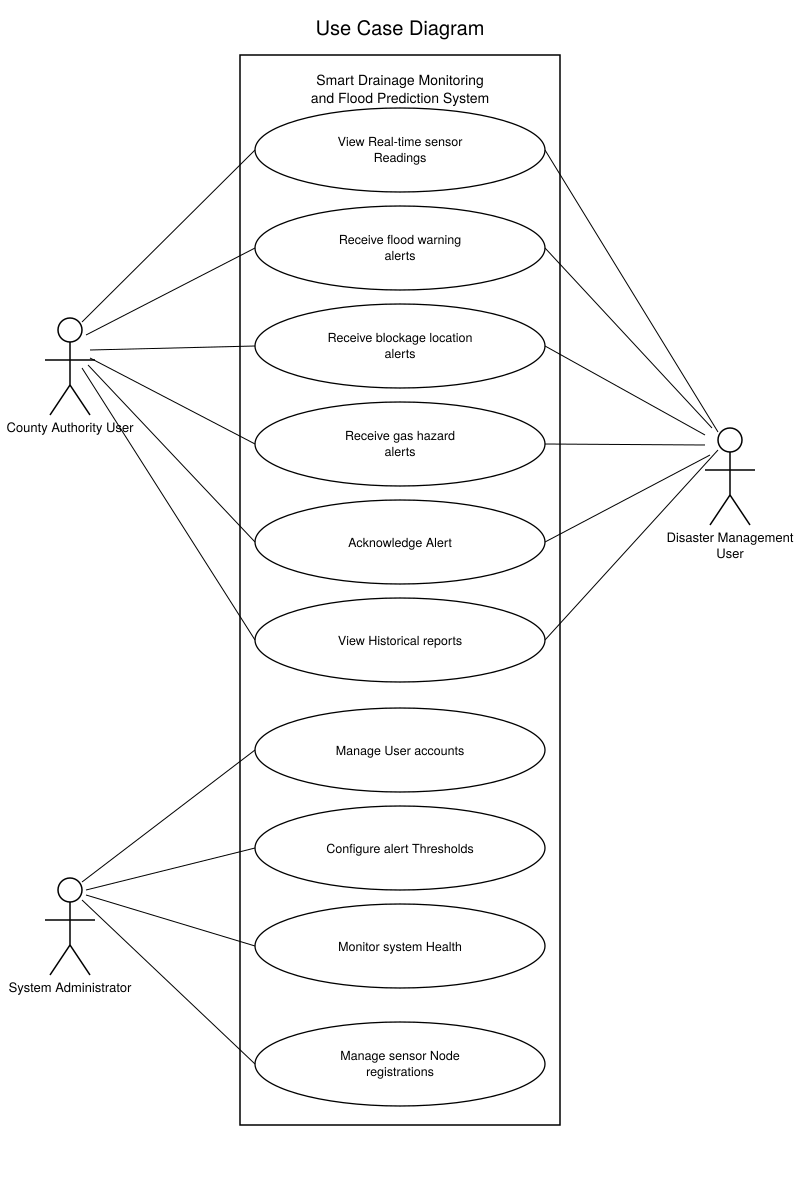
\includegraphics[width=0.8\textwidth]{Images/use_case_diagram.png}
    \caption{Use Case Diagram}
    \label{fig:use_case_diagram}
\end{figure}
\clearpage
 
\subsection{Class Diagram}
 
The diagram contains nine classes. The \texttt{SensorNode} class represents a physical monitoring node and provides methods for registering the node and updating its operational status. The \texttt{SensorReading} class represents a single timestamped data record transmitted from a node. The \texttt{AnomalyDetector} class implements the Isolation Forest anomaly detection stage, the \texttt{DrainageClassifier} class implements the Random Forest classification stage, and the \texttt{FloodPredictor} class implements the LSTM prediction stage; each of these three classes exposes the model-specific method used to process a sensor reading. The \texttt{Alert} class represents a system-generated notification, the \texttt{User} class manages system accounts and authentication, and the \texttt{Report} class represents a generated analytical report.
 
The ninth class, \texttt{ModelConfiguration}, was introduced to hold the operating parameters (model type, threshold, version, training date, and active status) used by the three machine learning classes at runtime. Rather than being hard-coded, each of \texttt{AnomalyDetector}, \texttt{DrainageClassifier}, and \texttt{FloodPredictor} holds a one-to-one \emph{uses} association with \texttt{ModelConfiguration}, allowing the anomaly threshold, classifier version, and prediction model to be retrained and updated without modifying application code. This directly supports the feedback and calibration loop shown in the System Architecture diagram (Section 4.6).
 
The remaining relationships are as follows. \texttt{SensorNode} has a one-to-many \emph{generates} association with \texttt{SensorReading}. \texttt{SensorReading} is analysed by \texttt{AnomalyDetector}, which is in turn classified by \texttt{DrainageClassifier}, which is predicted by \texttt{FloodPredictor}; these three pipeline stages are modelled as sequential dependencies reflecting the one-directional flow of data through the pipeline. \texttt{FloodPredictor} has a one-to-many \emph{triggers} association with \texttt{Alert}, while \texttt{SensorNode} separately has a one-to-many \emph{concerns} association with \texttt{Alert}, distinguishing the node an alert is about from the pipeline stage that generated it. \texttt{User} has a one-to-many \emph{acknowledged by} association with \texttt{Alert} and a one-to-many \emph{generates} association with \texttt{Report}.
 
\begin{figure}[H]
    \centering
    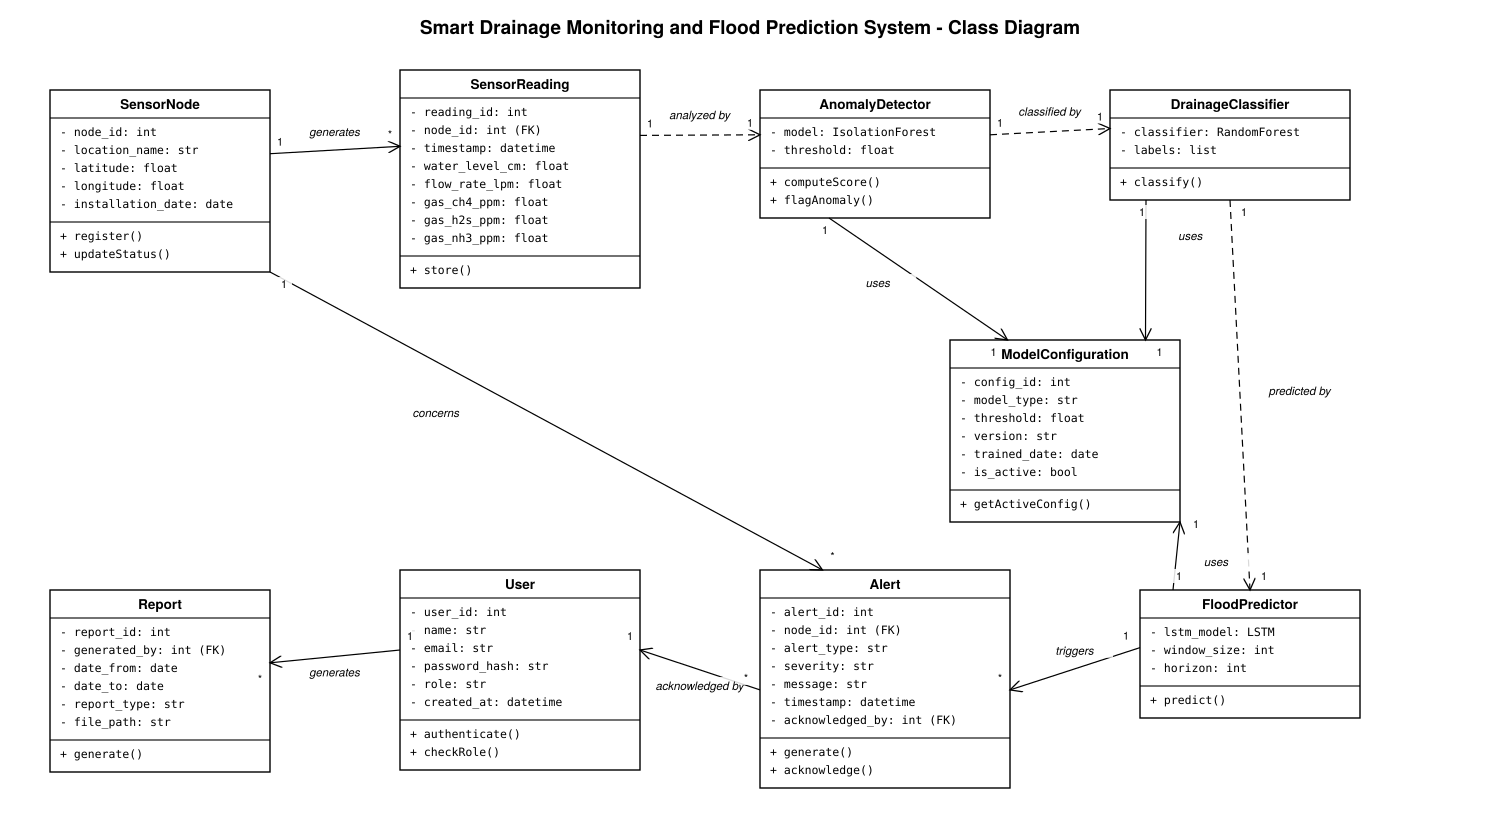
\includegraphics[width=\textwidth]{Images/class_diagram.png}
    \caption{Class Diagram}
    \label{fig:class_diagram}
\end{figure}
 
\subsection{Entity Relationship Diagram}
 
The ERD contains six entities, each shown with its attributes as connected ovals and its primary key underlined. The \texttt{SensorNode}, \texttt{SensorReading}, \texttt{Alert}, \texttt{User}, and \texttt{Report} entities correspond directly to their counterparts in the class diagram.
 
The sixth entity, \texttt{ModelConfiguration}, holds the attributes \texttt{config\_id} (primary key), \texttt{model\_type}, \texttt{threshold}, \texttt{version}, \texttt{trained\_date}, and \texttt{is\_active}, mirroring the \texttt{ModelConfiguration} class. It participates in a one-to-many \textsc{Applied To} relationship with \texttt{Alert}, recording which model configuration version produced a given alert.
 
The relationships among the remaining entities are as follows: \texttt{SensorNode} \textsc{Generates} \texttt{SensorReading} (one-to-many); \texttt{SensorNode} \textsc{Concerns} \texttt{Alert} (one-to-many), a relationship named to reflect that the sensor node is the subject of the alert rather than its cause; \texttt{User} \textsc{Acknowledges} \texttt{Alert} (one-to-many); and \texttt{User} \textsc{Produces} \texttt{Report} (one-to-many).
 
\begin{figure}[H]
    \centering
    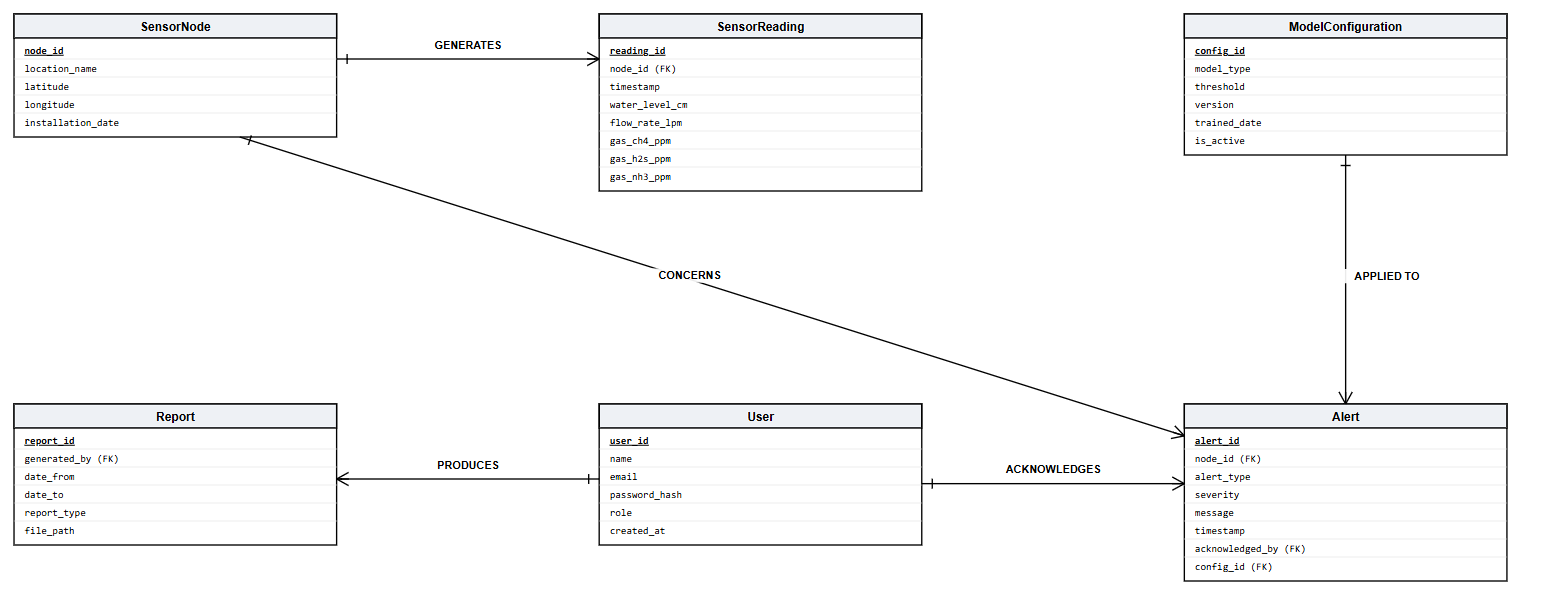
\includegraphics[width=\textwidth]{Images/erd_diagram.png}
    \caption{Entity Relationship Diagram}
    \label{fig:erd_diagram}
\end{figure}
 
\subsection{Database Schema}
 
The schema comprises six tables: \texttt{sensor\_nodes}, \texttt{sensor\_readings}, \texttt{alerts}, \texttt{users}, \texttt{reports}, and \texttt{model\_configurations}. The full column-level structure, data types, and constraints for each table are presented in Section 3.4.4. The \texttt{model\_configurations} table was added to persist the runtime parameters of the three machine learning pipeline stages, and the \texttt{alerts} table carries a nullable \texttt{config\_id} foreign key referencing it, so that every generated alert can be traced back to the exact model version that produced it.
 
\begin{figure}[H]
    \centering
    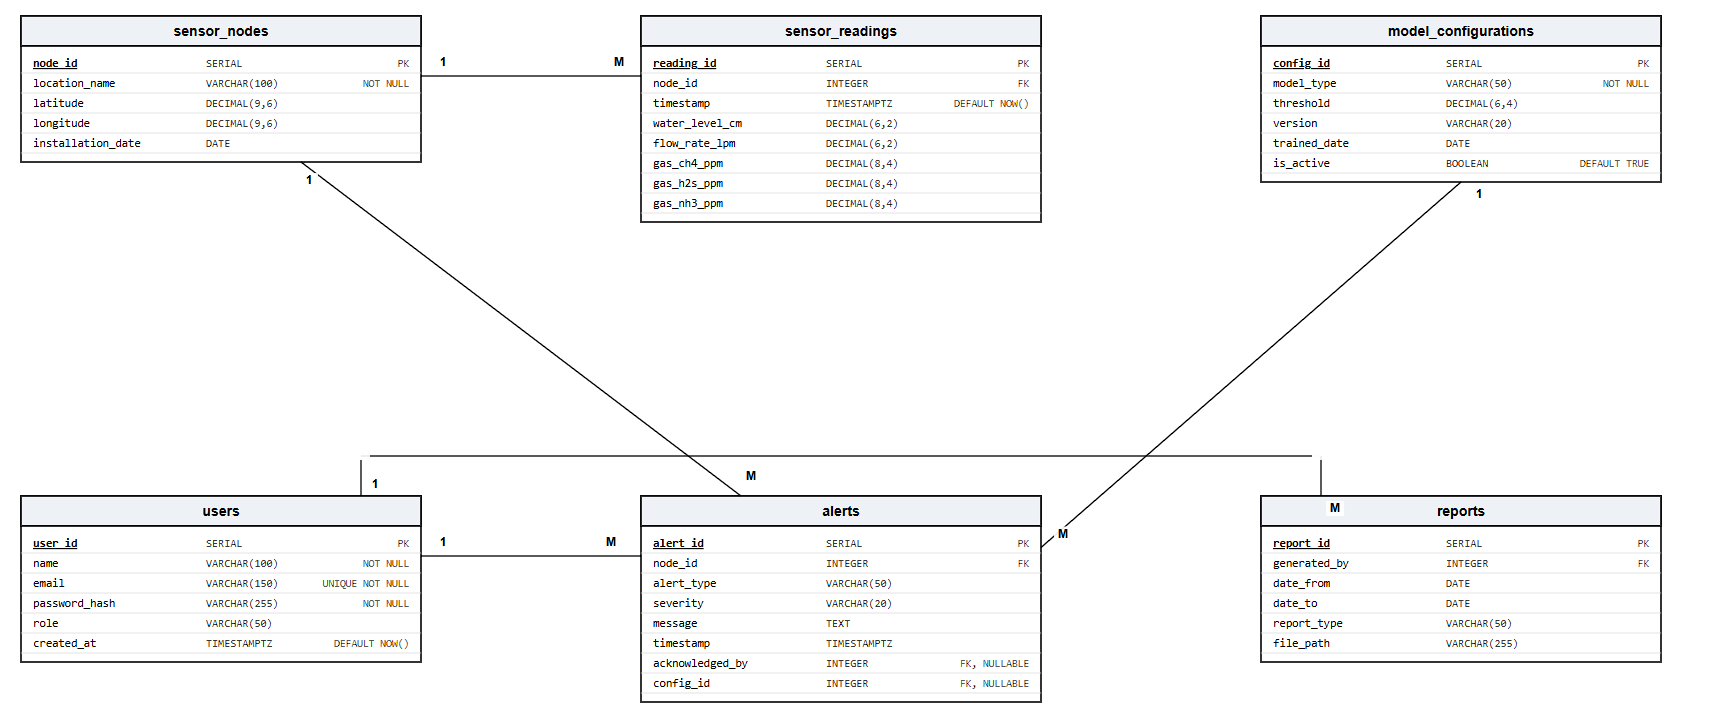
\includegraphics[width=\textwidth]{Images/database_schema.png}
    \caption{Database Schema }
    \label{fig:database_schema}
\end{figure}
 
\subsection{System Architecture}
 
The architecture is organised into three tiers that collectively handle data collection, processing, and presentation.
 
The sensing layer consists of ESP32-based sensor nodes deployed at multiple monitoring points across the drainage network; each node is fitted with an ultrasonic water level sensor, a flow rate sensor, and MQ-series gas sensors for methane, hydrogen sulfide, and ammonia. Each node publishes its readings as JSON payloads over MQTT via Wi-Fi.
 
The processing layer consists of an MQTT broker, a Python (Flask/Django) backend server, a PostgreSQL database, and the three-stage machine learning pipeline. The backend ingests incoming sensor payloads into the database. The pipeline reads sensor readings and the active model configuration from the database, passing each reading through the Isolation Forest anomaly detector, the Random Forest drainage-state classifier, and the LSTM flood predictor in sequence, and writes the resulting classifications and predictions back to the database. A feedback and calibration loop allows updated thresholds and retrained model versions to be written back to the \texttt{model\_configurations} table without redeploying the pipeline code.
 
The presentation layer consists of the web-based monitoring dashboard, accessed over HTTPS by the County Authority User, the Disaster Management Agency User, and the System Administrator. The dashboard displays real-time sensor readings, active alerts with severity levels, flood warnings with time-to-threshold estimates, blockage and gas hazard alerts, and historical analytical reports.
 
\begin{figure}[H]
    \centering
    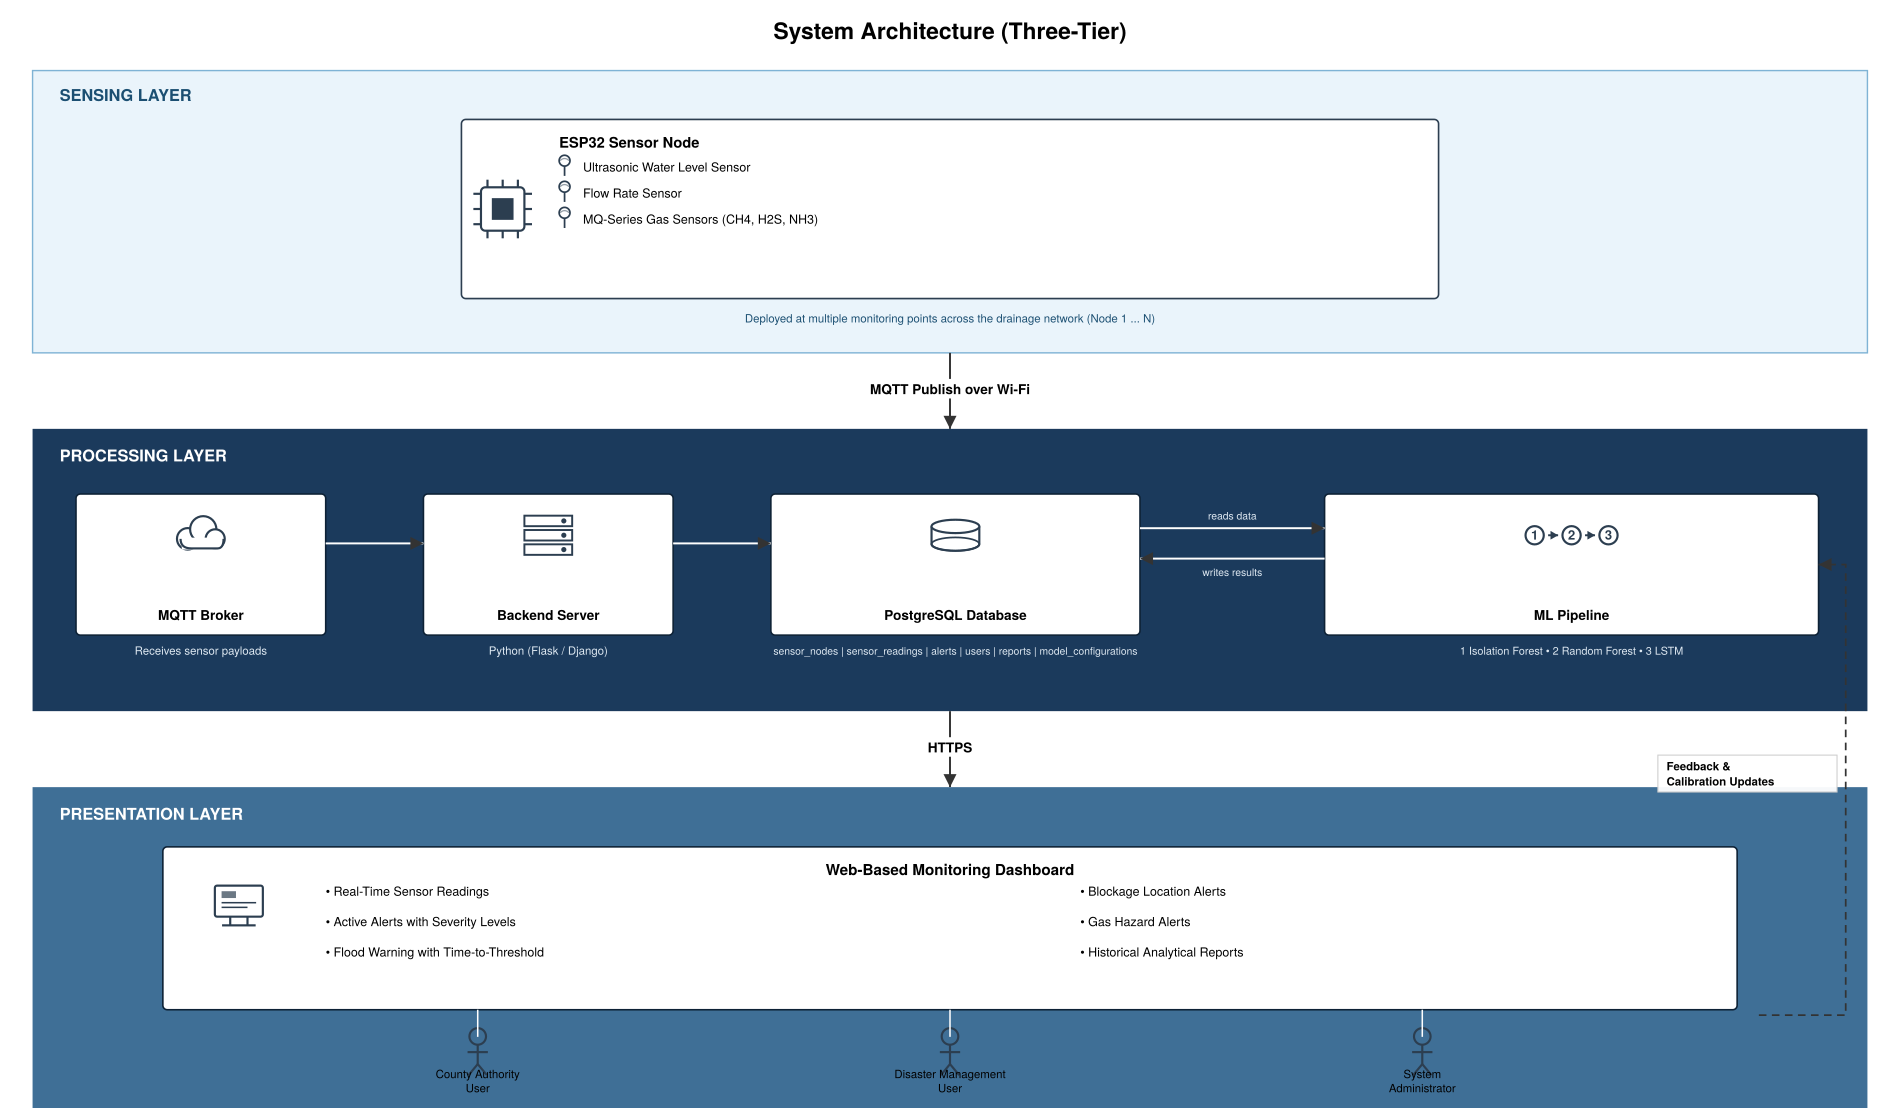
\includegraphics[width=\textwidth]{Images/system_architecture.png}
    \caption{System Architecture}
    \label{fig:system_architecture}
\end{figure}
 
\subsection{Wireframes}
 
The wireframes cover four primary screens. The main monitoring dashboard screen is the default landing screen for all authenticated users and is divided into four panels: a navigation bar showing the system name, current user, and role; a node status map showing the geographic positions of all registered sensor nodes along the monitored drainage channel, colour-coded green for Normal, amber for Blockage Risk, and red for Flood Risk; a live sensor readings table listing each node's most recent readings and current state; and an active alerts panel listing the most recent unacknowledged alerts.
 
\begin{figure}[H]
    \centering
    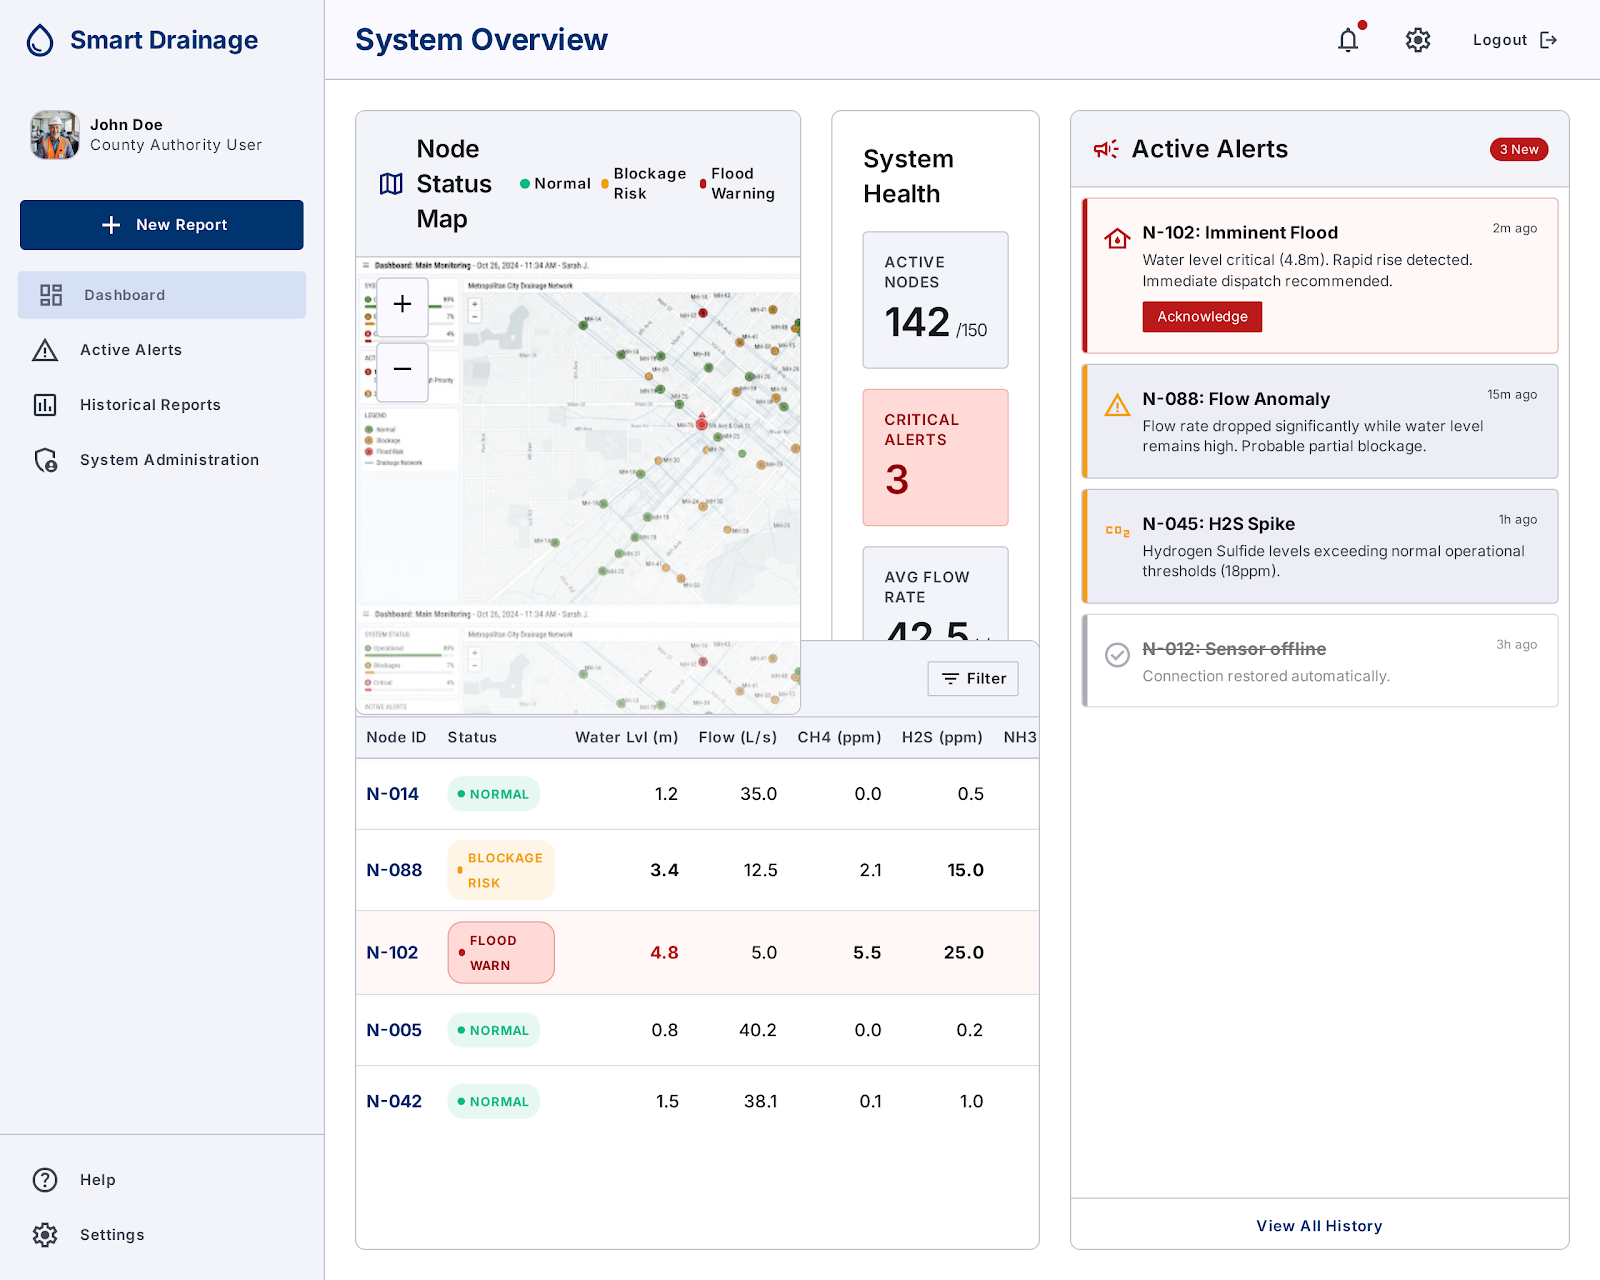
\includegraphics[width=\textwidth]{Images/wireframe_dashboard.png}
    \caption{Main Monitoring Dashboard Wireframe}
    \label{fig:wireframe_dashboard}
\end{figure}
 
The alert detail screen displays the complete alert record, including the alert type, severity, affected node, the sensor readings that triggered it, the output of each of the three machine learning pipeline stages together with the model configuration version used to produce them, a recommended action, and an acknowledgement button that records the acknowledging user and timestamp against the alert.
 
\begin{figure}[H]
    \centering
    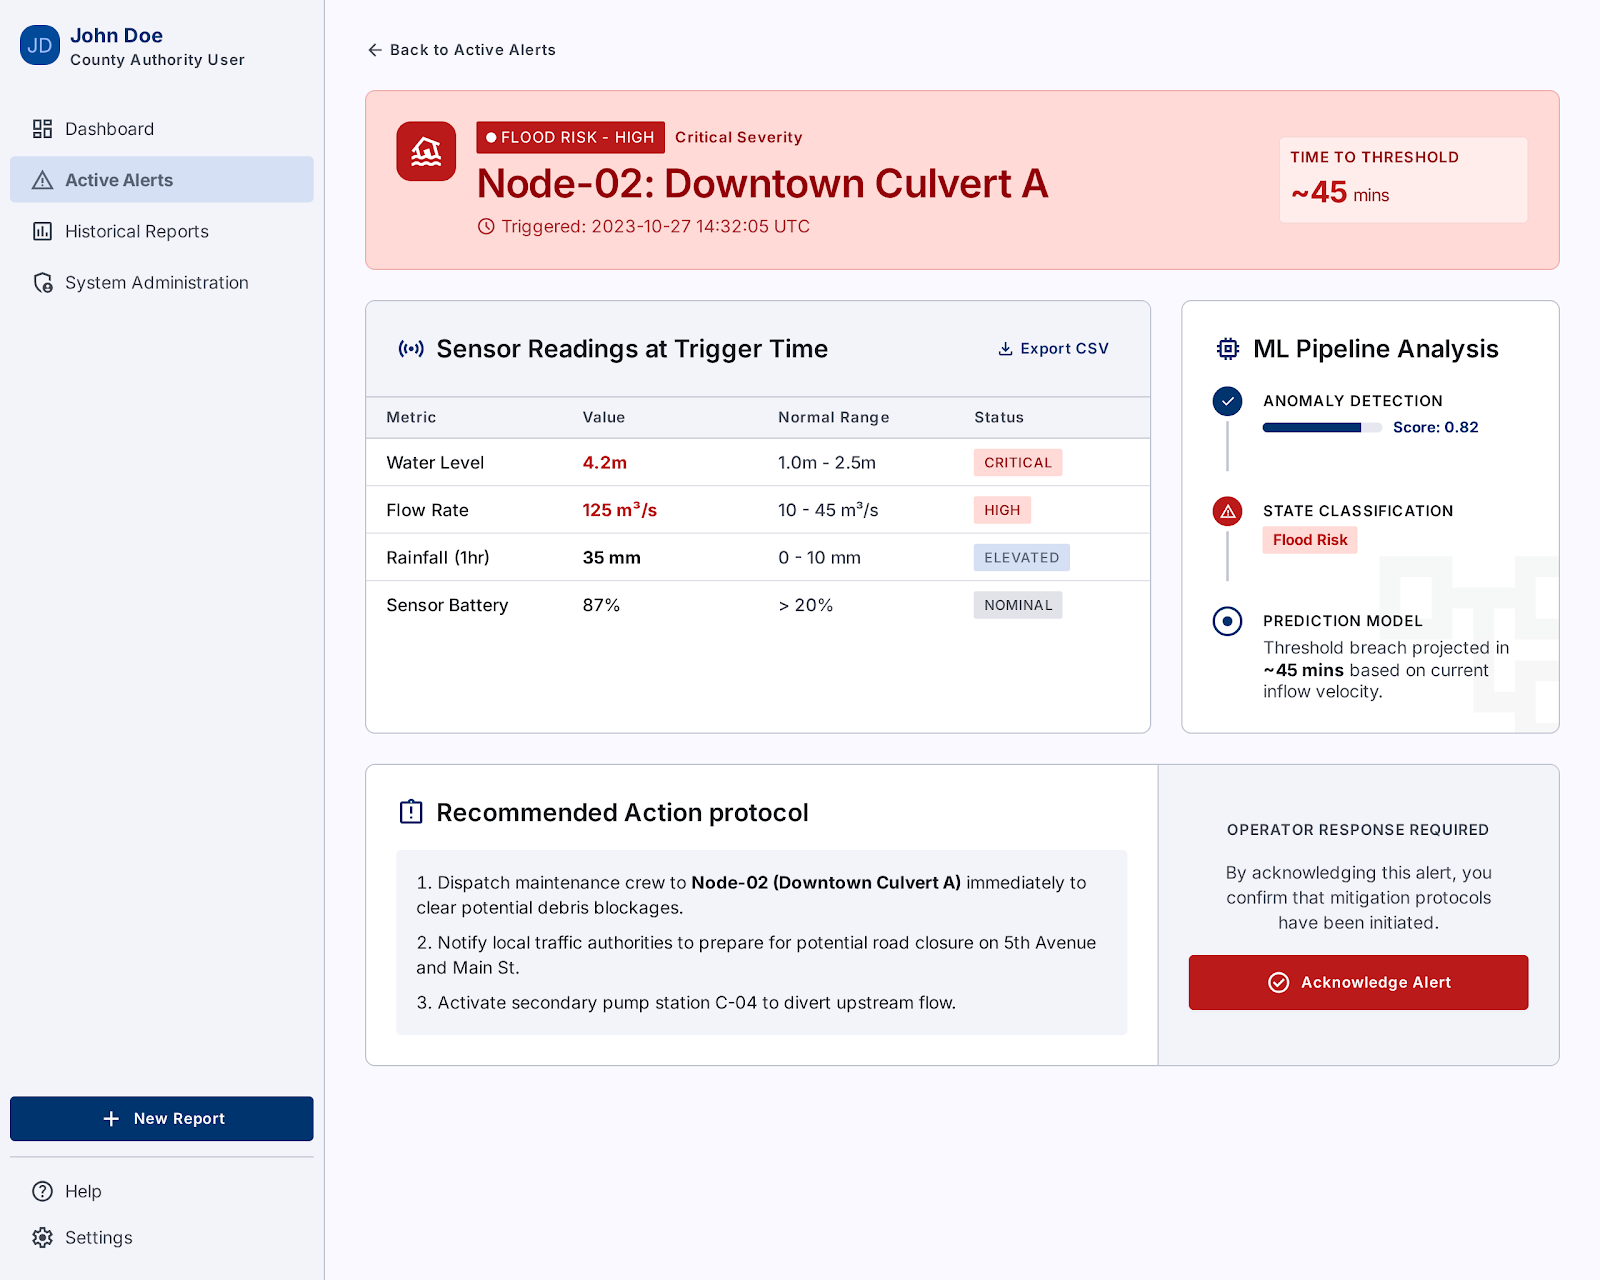
\includegraphics[width=\textwidth]{Images/wireframe_alert_detail.png}
    \caption{Alert Detail Wireframe}
    \label{fig:wireframe_alert_detail}
\end{figure}
 
The historical reports screen provides a form for generating reports by date range, sensor node, and report type (Sensor Summary, Alert History, or ML Performance), together with a table of previously generated reports available for download.
 
\begin{figure}[H]
    \centering
    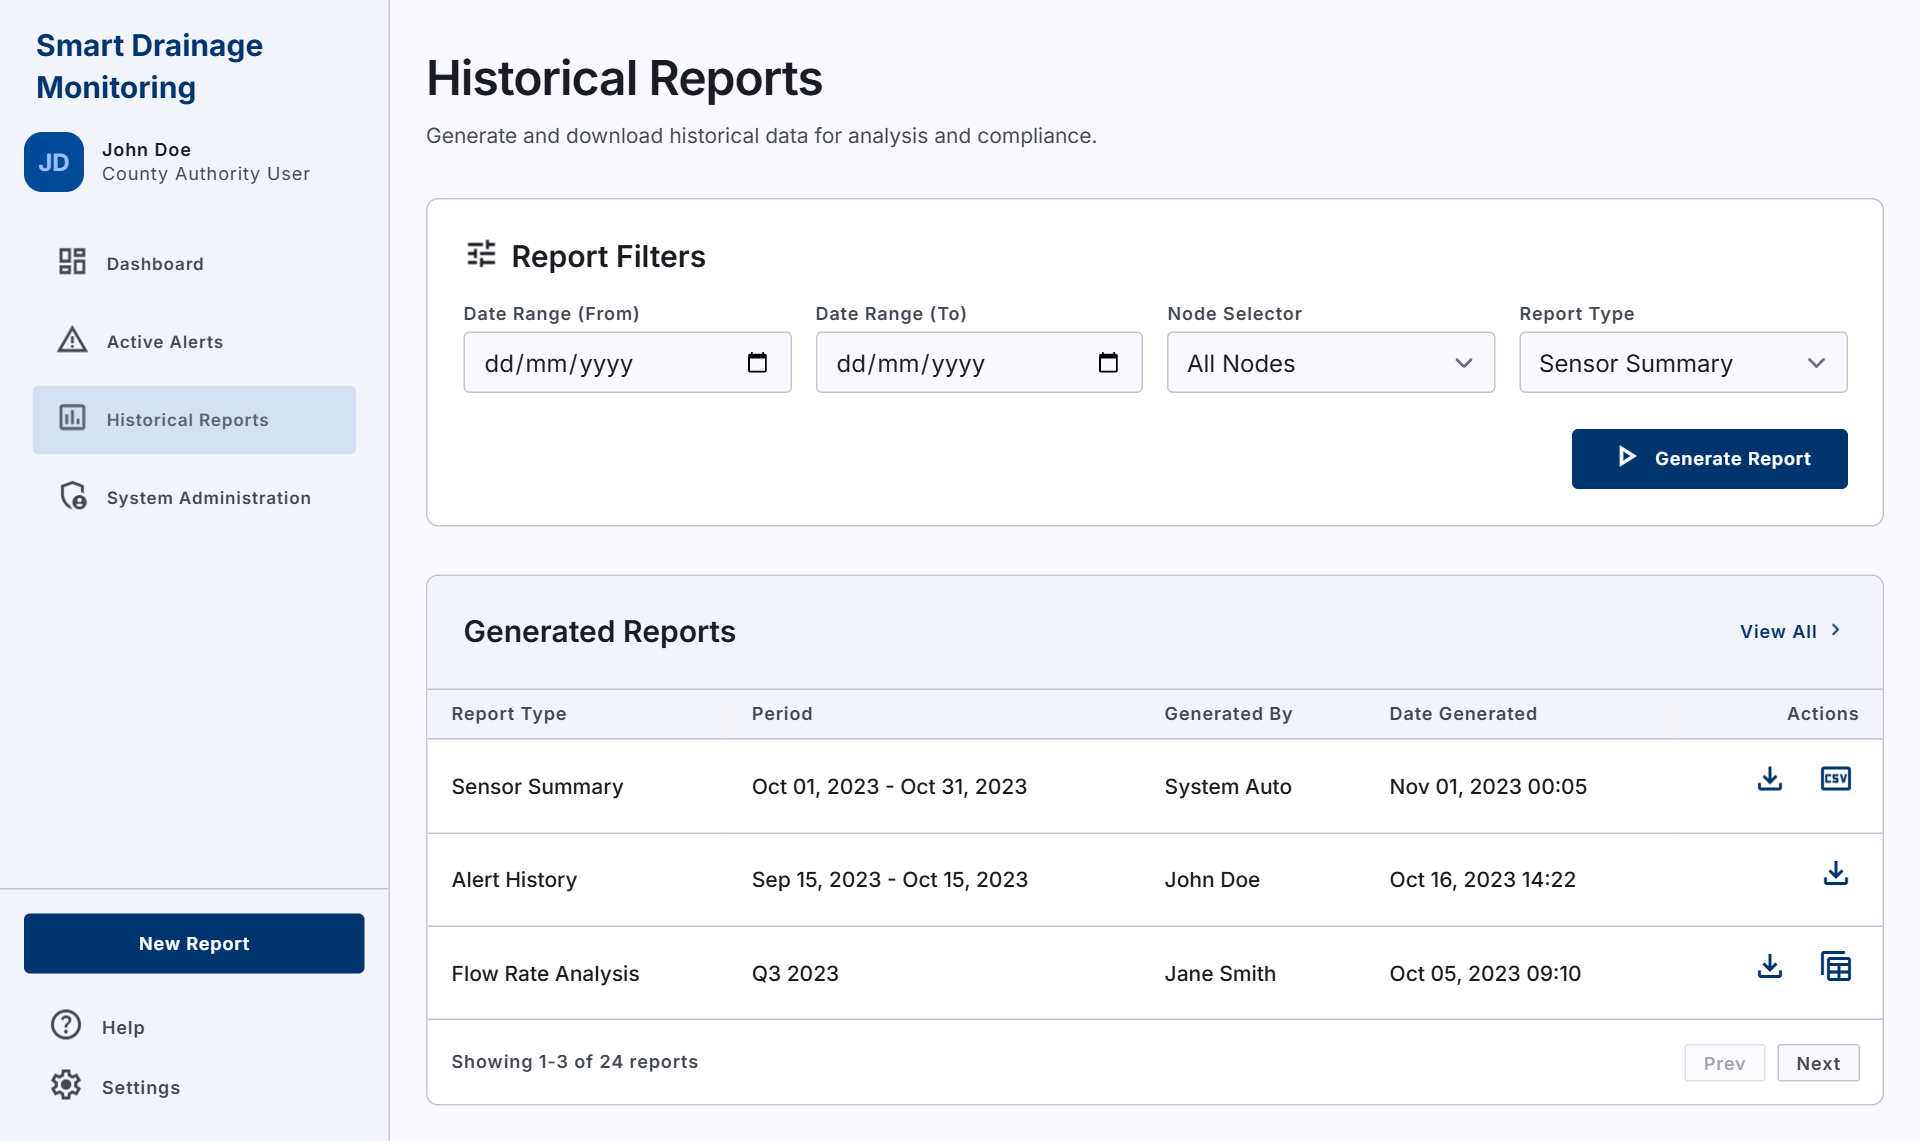
\includegraphics[width=\textwidth]{Images/wirefame_reports.png}
    \caption{Historical Reports Wireframe}
    \label{fig:wireframe_reports}
\end{figure}
 
The system administration screen is accessible only to the System Administrator role and contains four tabbed sections: user account management, alert threshold configuration, sensor node management, and model configuration, the last of which allows the model type, threshold, version, training date, and active status of each of the three pipeline stages to be reviewed and updated.
 
\begin{figure}[H]
    \centering
    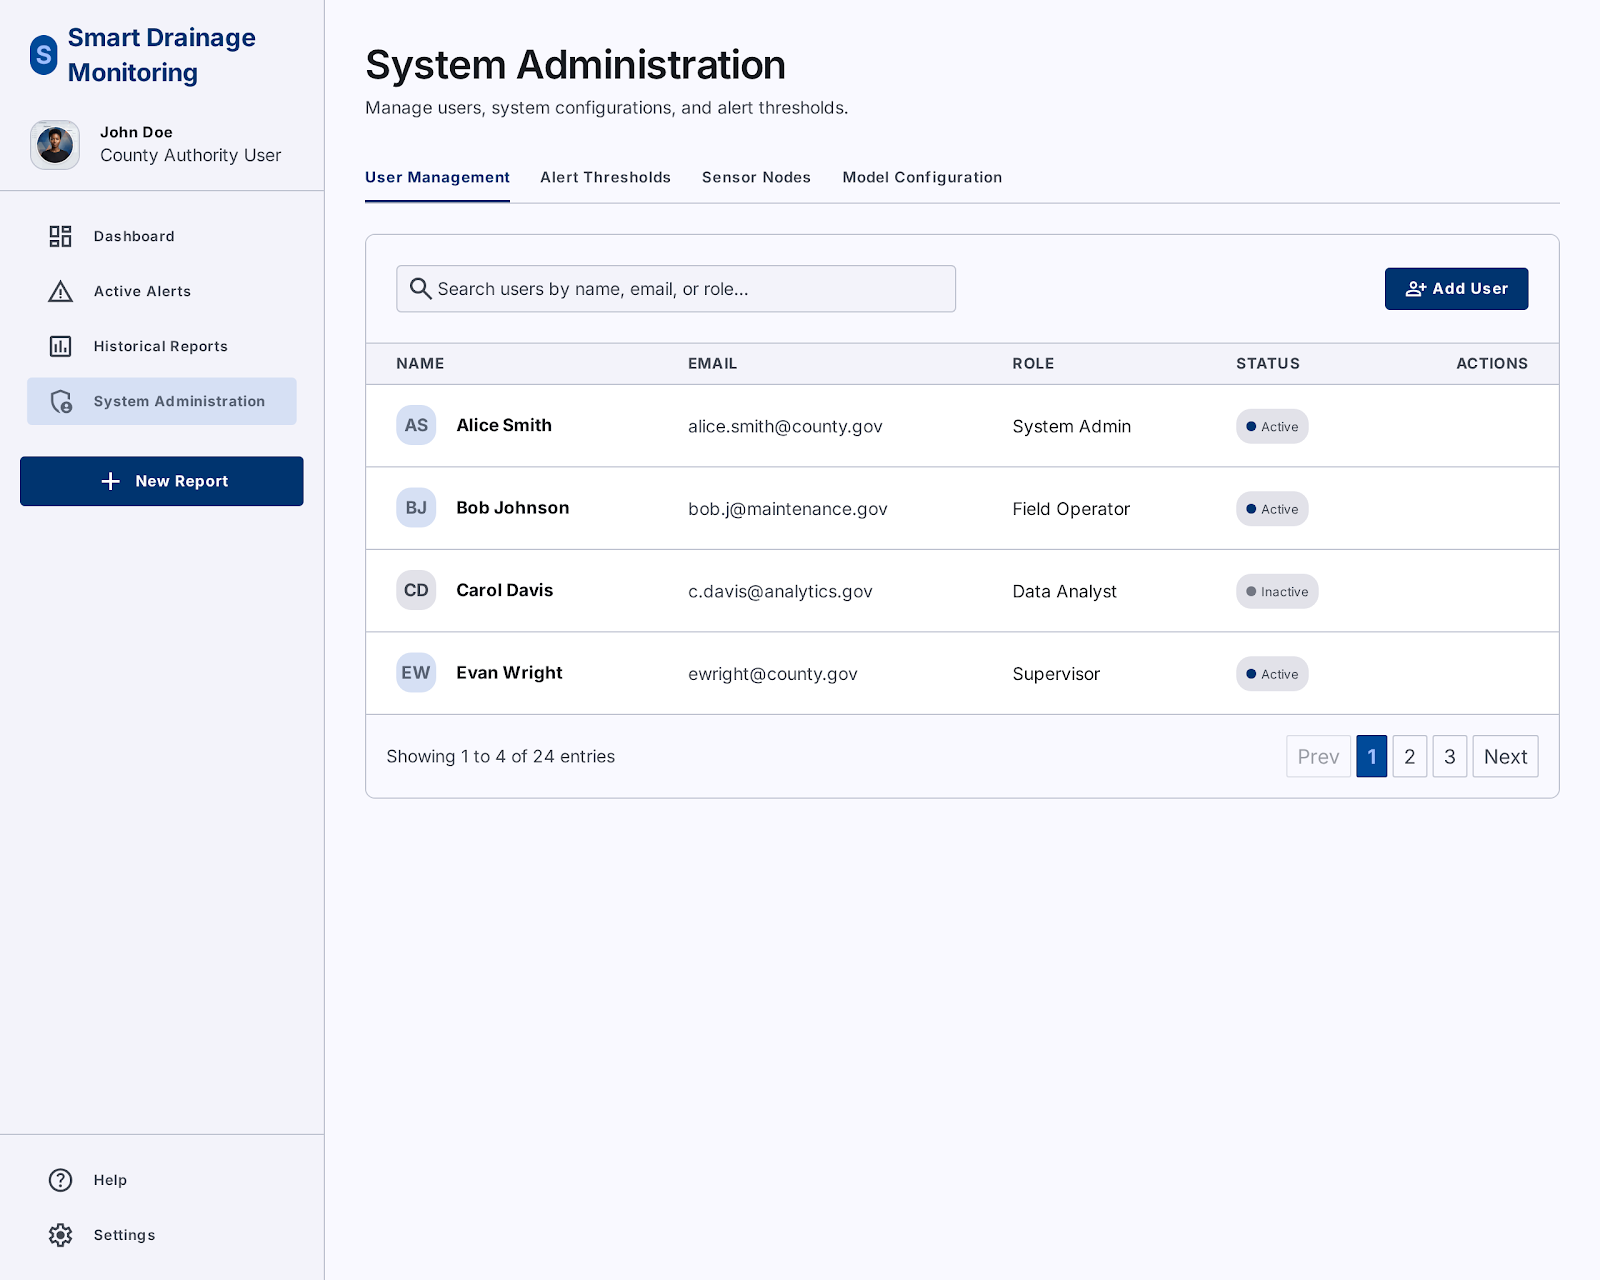
\includegraphics[width=\textwidth]{Images/wireframe_admin.png}
    \caption{System Administration Wireframe}
    \label{fig:wireframe_admin}
\end{figure}
\clearpage

\bibliographystyle{apalike}
\bibliography{bibliography}

\clearpage
\section*{Appendices}
\addcontentsline{toc}{section}{Appendices}

\renewcommand{\thefigure}{A\arabic{figure}}
\setcounter{figure}{0}

\subsection*{Appendix A: Agile Project Timeline}

\begin{figure}[H]
    \centering
    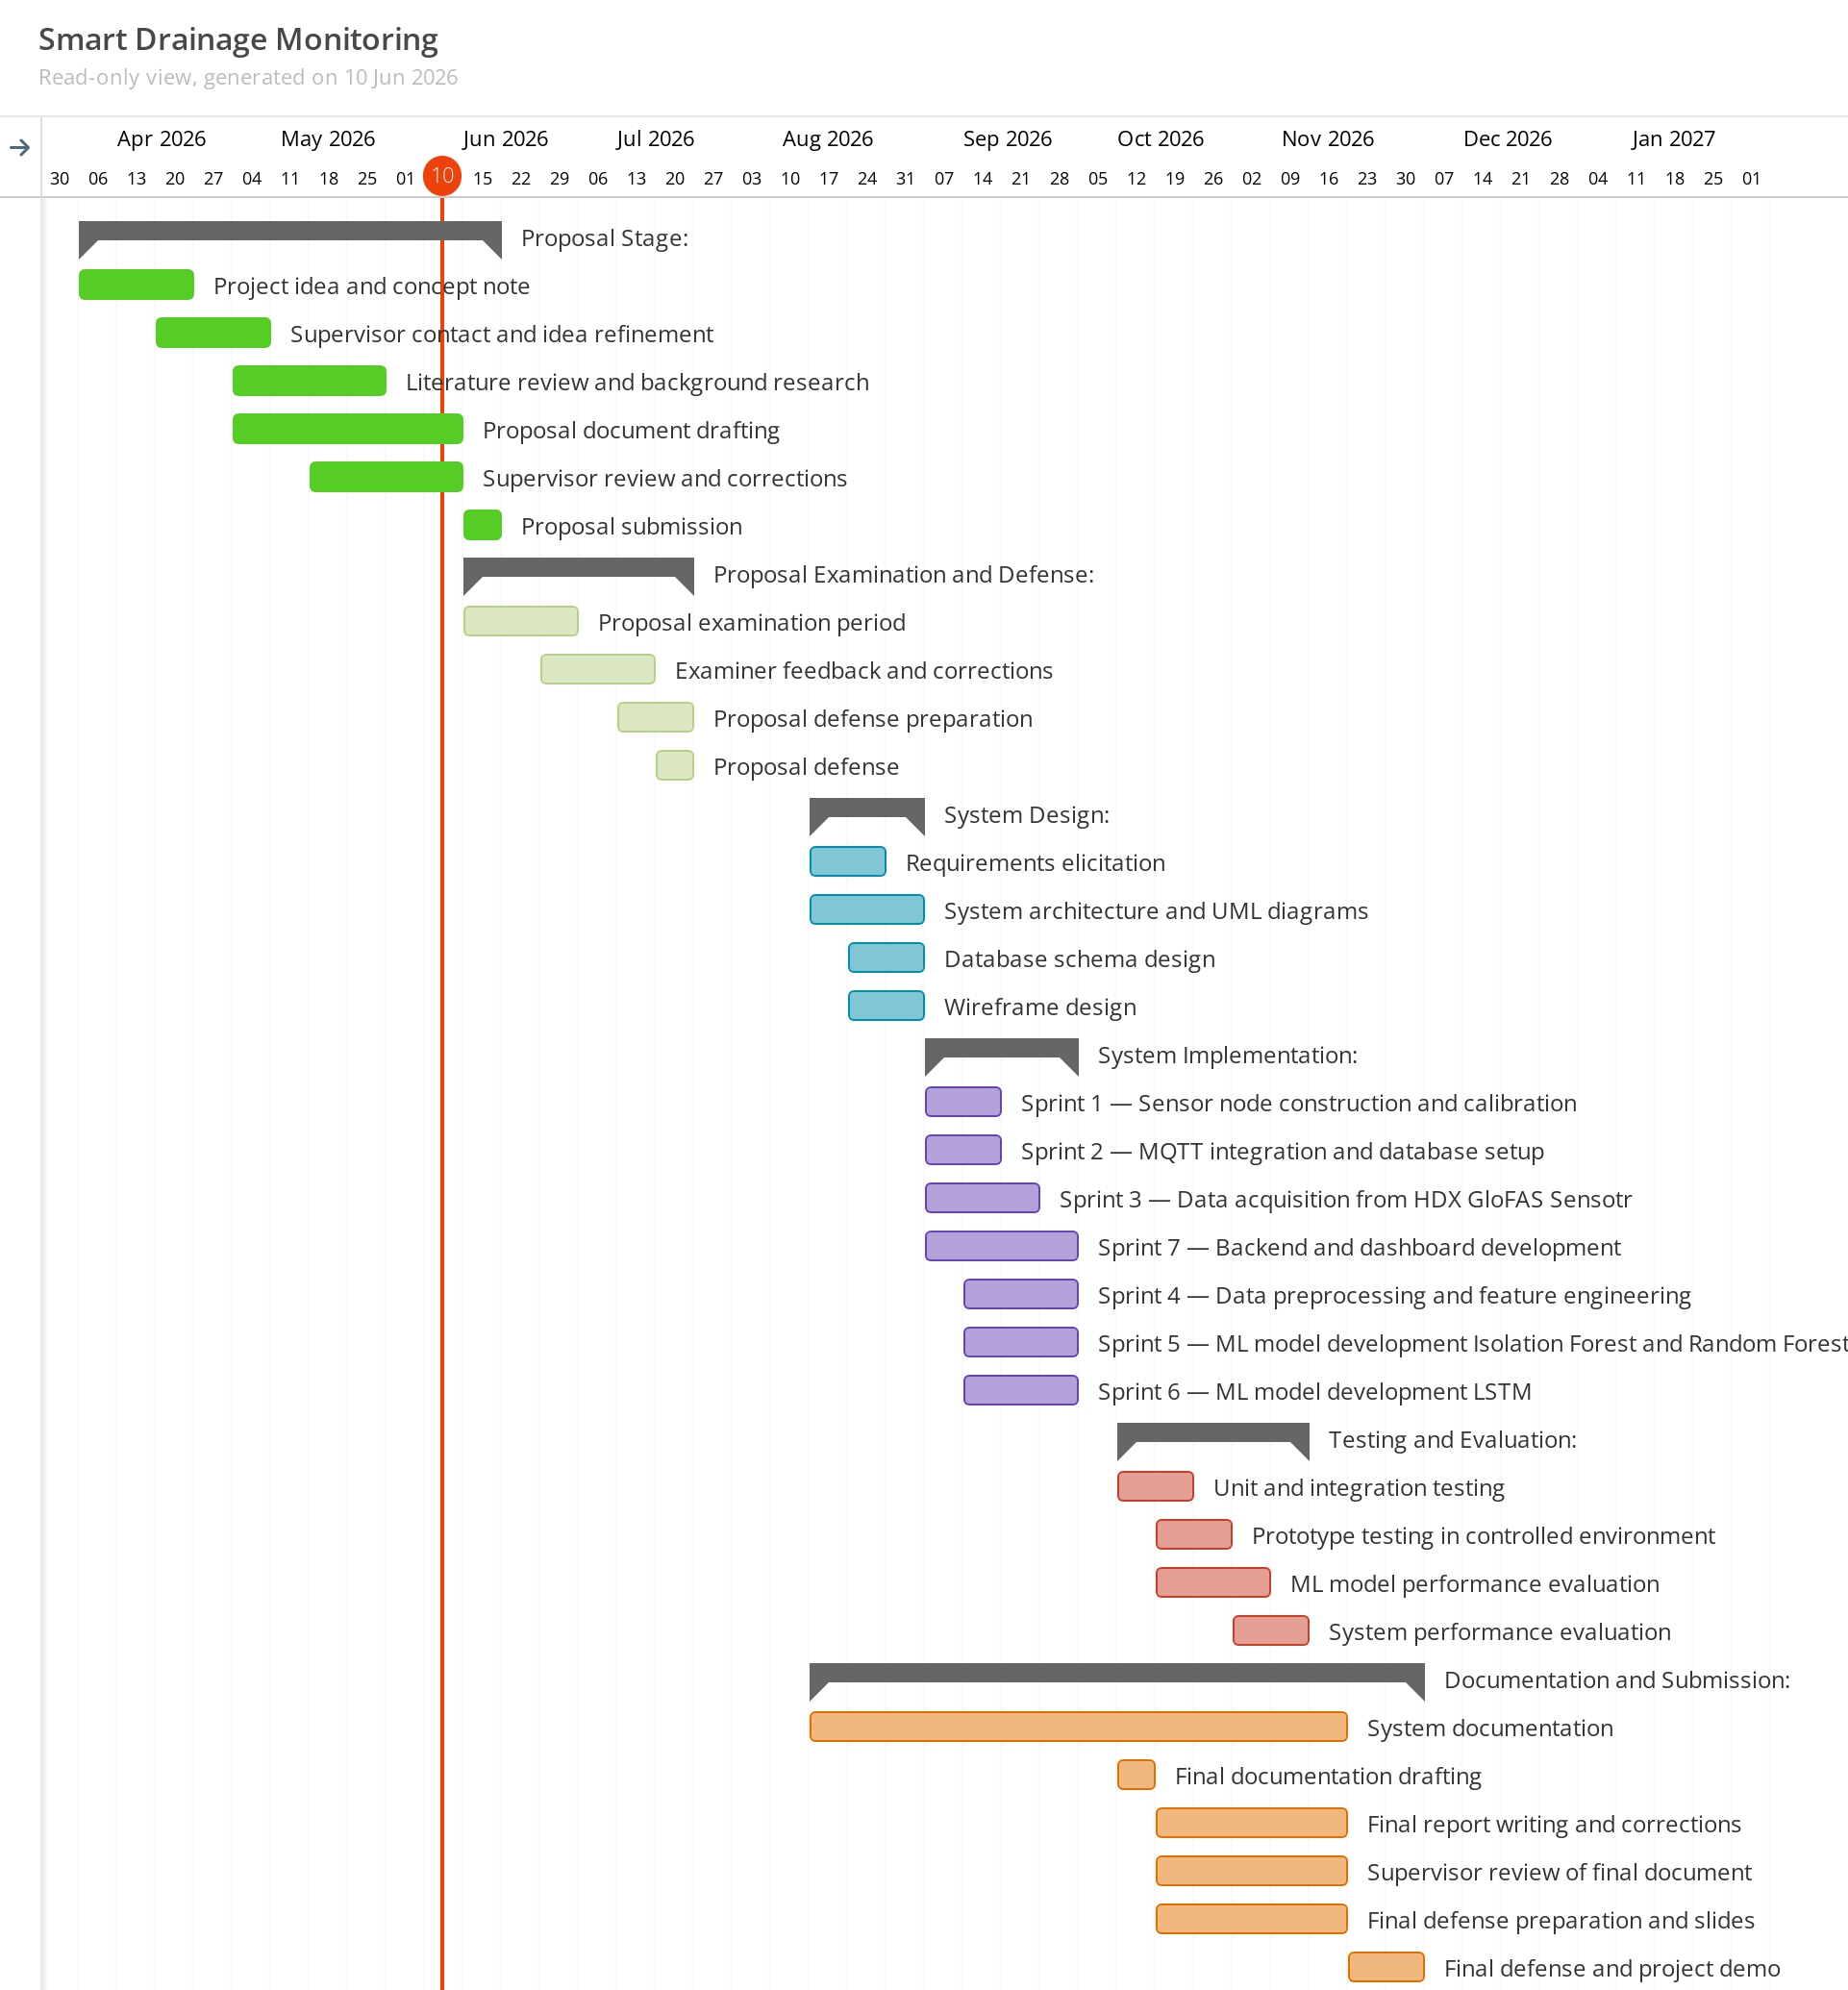
\includegraphics[width=\textwidth]{Images/gantt_chart.png}
    \caption{Agile Project Timeline for the Smart Drainage Monitoring 
    and Flood Prediction System}
    \label{fig:gantt_chart}
\end{figure}

\clearpage
\subsection*{Appendix B: Turnitin Similarity Report}

\begin{figure}[H]
    \centering
    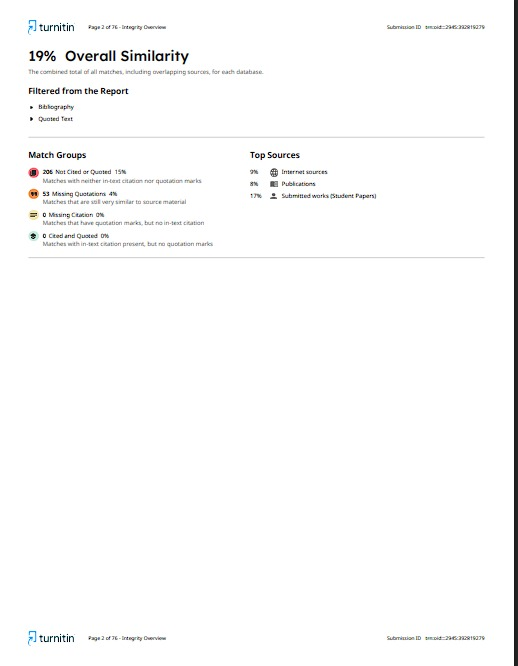
\includegraphics[width=\textwidth]{Images/turnitin.png}
    \caption{Turnitin Similarity Report for the Smart Drainage Monitoring 
    and Flood Prediction System Proposal}
    \label{fig:turnitin_report}
\end{figure}
 
\end{document}